\documentclass{book}
% math formatting
\usepackage{amssymb, amsmath}

% Code formatting
\usepackage{helvet}     % Julian called out Helvetica font for code
\usepackage{pxfonts}    % Bold inline code
\usepackage{listings}
    \lstset{escapeinside={(*@}{@*)} , % allow footnote in listing
            basicstyle=\ttfamily }
\newcommand{\bc}[1]{\textbf{\lstinline{#1}}}
\newcommand{\regc}[1]{\lstinline{#1}}
% For code in paragraphs use \lstinline$word$
% For bolded code in paragraphs use \bc{word}
% For code not in paragraphs use \begin{listing} code here \end{listing}

% Extend the footnote line across the page
\makeatletter
\renewcommand\footnoterule{%
  \kern-3\p@
  \hrule\@width \textwidth
  \kern2.6\p@}
\makeatother

\let\cleardoublepage\clearpage

% Place a blank line with every space between paragraphs
\edef\restoreparindent{\parindent=\the\parindent\relax}
\usepackage{parskip}
  \restoreparindent

% Have a paragraph's first letter span 2 lines
\usepackage{lettrine}
    \newcommand{\TallC}[2]{\lettrine[lines=2]{\textbf{#1}}{#2}}
% \TallC{T}{he} to create a large T

% Dotted lines across the page
\newcommand{\dotrule}[1]{%
   \parbox[t]{#1}{\dotfill}}
% \dotrule{1\textwidth} will make it across the page

% Side bar at some points in the text
\usepackage{framed}
\renewenvironment{leftbar}[1][\hsize]
{%
    \def\FrameCommand
    {%
        {\vrule width 2pt}%
        \hspace{0pt}%must no space.
        % \fboxsep=\FrameSep\colorbox{yellow}%
    }%
    \MakeFramed{\hsize#1\advance\hsize-\width\FrameRestore}%
}
{\endMakeFramed}
% Use \leftbar[1\linewidth] at the beginning
% Ues \endleftbar at the end

%Highlight cell color
\usepackage[table]{xcolor}
    \newcommand{\lgray} {\cellcolor[HTML]{D3D3D3}}
    \newcommand{\Aggray}{\cellcolor[HTML]{C0C0C0}}
    \newcommand{\gray}  {\cellcolor[HTML]{808080}}
    \newcommand{\dgray} {\cellcolor[HTML]{A9A9A9}}
    \newcommand{\digray}{\cellcolor[HTML]{696969}}
% use \cellcolor[HTML]{AA0044} in the prefered cell

%Create charts with tikz
\usepackage{tikz}
\usetikzlibrary{shapes.geometric, arrows}
    \tikzstyle{wordinr1} = [rectangle, text centered, draw=black]
    \tikzstyle{wordinr2} = [rectangle, text centered, draw=black, minimum width=1.5cm]
    \tikzstyle{arrow}   = [thick,->,>=stealth]

%Prefixing chapter/section numbers with ยง
\usepackage{cleveref}
  \crefname{section}{\S}{\S\S}
  \Crefname{section}{\S}{\S\S}
  \crefformat{section}{\S#2#1#3}

%Mini table of contents
\usepackage{titlesec}
\usepackage{titletoc}

%Thinking FORTH
\newcommand{\TF}{\textbf{TF}}
%Starting FORTH
\newcommand{\SF}{\textbf{SF}}
%FORTH: a Text and Reference
\newcommand{\FTR}{\textbf{FTR}}
%e.g. in italics
\newcommand{\eg}{\textit{e.g.}}
%Note
\newcommand{\Note}{\textbf{\underline{Note}}}

%Current Chapter on which you are working.
\includeonly{Chapter-04/04-The-80x87-Family}

\begin{document}
\tableofcontents
%\chapter{Toward Scientific FORTH}
\TallC{This} book presents extensions to the FORTH programming language suitable for scientific and technical computation. The aim is to retain FORTRAN s good points while taking advantage of the simplicity, flexibility, extensibility, and control offered by FORTH.

The resulting dialect has many advantages over more traditional languages, both for small, casual, throw-away programs as well as for large, complex projects. FORTH lends itself to many programming styles, including procedural, object oriented or event-driven. Its speed and economical use of memory suit FORTH for real-time, on-line data pre-processing well as as off-line analysis and computation.

Because FORTH is a \textbf{threaded, interpretive} language\sepfootnote{01_01} its  structure and philosophy differ radically from those of traditional languages like FOTRAN and BASIC. This introductory chapter explains some of the differences by contrasting FORTRAN with FORTH.

\section{Overview of FORTRAN}
\TallC{FORTRAN} is a \textbf{compiled} high level language\sepfootnote{01_02}. The programmer writes a \textbf{source code} program using FORTRAN's grammatical rules, data structures and operators; a special computer program (the \textbf{compiler}) then translates the source into a (relocatable) machine language version (\textbf{object code}). Another machine language program (the \textbf{linker}) then links modules of object code into an \textbf{executable} program that can be run under the control of the operating system of the computer.

Compilation produces executable programs that run fast, without the tedium of writing them directly in machine code (or \textbf{assembly language}). The source code will run virtually the same on any machine for which a compiler exists. That is, the source code is \textbf{portable}. Among other things, portability makes possible the development of standard libraries of reusable code for performing standard tasks like solving linear equations or computing Bessel functions.

The chief disadvantage of compilation is its tedium. Testing small portions of a program in isolation is virtually impossible -- either an "exercise" program must be written and compiled with the module being tested, or else the entire program must be compiled as a unit. This process is so time-consuming it discourages fine-grained decomposition of programs into small, comprehensible components.
 
\subsection{Programs and sub-programs} 
\TallC{A} FORTRAN program consists of a master, or \textbf{main} program that either stands alone or can \textbf{call} (transfer control to) sub-programs. Sub-programs fall into two classes: \textbf{subroutines} and \textbf{functions}. Both receive \textbf{arguments} (input) from the calling program; they differ in how \textbf{results} (output) are returned to the calling program. Subroutines are called by the phrase

\begin{verbatim}
CALL SUB1(A,B,RESULT)
\end{verbatim}

where \verb|A| and \verb|B| are arguments and \verb|RESULT| is the result (which is returned in the argument list). By contrast, a function is called by having its name placed in an arithmetic expression. When the expression is evaluated, the value of the function (at its given arguments) is inserted in the expression where the function name appeared. That is, we might have a phrase like

\begin{verbatim}
OPSIDE = HYPOT*SIN(3.14159*ANGLE/180.).
\end{verbatim}

Here the argument of \verb|SIN| is also an expression which must be evaluated before being passed to the \verb|SIN| subroutine. When \verb|SIN| is evaluated, its value is returned, multiplied by \verb|HYPOT| and the product stored in the area labelled \verb|OPSIDE|.

There is no specific calling hierarchy in FORTRAN -- a function an call a subroutine or \textit{vice-versa} and the called sub-program can all still further sub-programs.

\subsection{Arithmetic statements}
\TallC{FORTRAN} arithmetic is performed by "smart" operators acting on \textbf{typed variables} and \textbf{literals}. A variable is simply a name that refers to a specific location in memory. The \textbf{type} declaration is a way to let the compiler know how much memory to allot for that variable. A literal is an explicit number that appears in the program, such as the values \verb|3.14159| and \verb|180|. in the preceding example.

FORTRAN arithmetic expressions can freely mix types. To make this possible, the arithmetic operators are \textbf{overloaded} in the sense that the plus sign --say-- can add floating point numbers, integers, or numbers in any combination, mixture or order.

Consider, \eg, the actions performed by the FORTRAN compiler in parsing the arithmetic assignment statement 

\begin{verbatim}
A = B1*3 + B2*1.2E-5 - H(3)/3.14159265358969D14 + K
\end{verbatim}

keeping in mind that FORTRAN, data types can be declared explicitly or implicitly\sepfootnote{01_03}:
\begin{itemize}
    \item Define and reserve space for floating-point single precision variable \verb|A| (implicit type REAL) if \verb|A| has not been defined previously (perhaps as something else);
    \item Convert the literal integer constant \verb|3| to floating point and multiply it by the (implicit-REAL) variable \verb|B1|'s current value (fetch from memory), placing the product in temporary storage (\verb|TEMP|).
    \item Fetch (implicit-REAL) variable \verb|B2| and multiply it by the REAL literal \verb|1.2E-s|;
    \item Add the second product to the contents Of \verb|TEMP|;
    \item Fetch the 3rd element of the (implicit-REAL) array \verb|H|;
    \item Divide by the DREAL (double-precision) literal \verb|3.14159265358979D-14| ($= \pi$ ), converting to and from DREAL format as necessary;
    \item Convert the dividend to REAL and subtract from \verb|TEMP|;
    \item Convert (implicit) INTEGER variable \verb|K| to REAL and add to \verb|TEMP|;
    \item Move the result from \verb|TEMP| to the memory reserved for \verb|A|.
\end{itemize}

These actions can be over-ridden by explicit type declarations. For example, if the program had contained the following statements in its first few lines:
\begin{verbatim}
    INTEGER A, H(15), B1, B2 
    REAL K
\end{verbatim}
the conversions and assignments would have been floating point to integer, rather than \textit{vice-versa}.

\TallC{To} achieve the simplicity of mixed-mode expressions, the FORTRAN compiler must be prepared for any eventuality. The operators "\textbf{+}", "\textbf{-}", "\textbf{*}", "\textbf{/}" and "\textbf{=}" must be "smart" (overloaded)-- they must "know" (or at least be able to figure out) what kinds of numbers are going to be used and what kinds of arithmetic will be used to combine them. The FORTRAN exponentiation operator "\textbf{**}" must similarly "know" whether the base is INTEGER, REAL DREAL or COMPLEX (some FORTRAN's even permit DCOMPLEX), and the same for the exponent. That is, it must be able to compile 16 (or 25) versions of \textbf{**}, depending on circumstances. The compiler must contain decision branches to handle every eventuality. Compilers for languages such as FORTRAN, PASCAL, C or Modula-2 are therefore complex and slow.

Smart operators benefit the user by simplifying source code. The benefit is only partial, however, since the programmer must still keep track of types in calling sequences for subroutines, and in declaring global variables with COMMON and EQUIVALENCE statements.
 
Since FORTRAN subroutines can be compiled separately, many a subtle bug has been introduced by omitting an argument from a long calling sequence, or by inverting arguments in a list (thereby, for example, telling a subroutine to interpret a REAL as a very large INIEGER). I can vouch for these problems from long, sad experience debugging FORTRAN.

FORTRAN provides a limited suite of data types: INTEGER, LONG-INTEGER, REAL, DREAL, COMPLEX, DCOMPLEX, LOGICAL and CHARACTER. It provides no facilities for defining any new types (other than arrays of the above). Arrays must be declared according to a strict format -- up to 3 indices are permitted.

FORTRAN's array notation is simple, logical and follows the conventions of algebra: parentheses replace subscripts \textit{via}

\begin{verbatim}
    A_{ij} => A(I,J).
\end{verbatim}

\TallC{FORTRAN} provides facilities for initializing constants and variables at run-time: the DATA statement within a program or subroutine, and the BLOCK DATA subprogram for initializing global variables in COMMON.

Limited control of memory allocation is provided: placed at the beginning of a program or subprogram, COMMON, BLOCK COMMON and EQUIVALENCE specification statements allow local variables to be made global or partially global, under the same or different names. DIMENSION allocates memory for arrays. (Dynamic re-allocation is not permitted.)

Finally, EXTERNAL directs the compiler (more precisely, the linker and loader) to search outside the subprogram for the specified name: for example, the usage

\begin{verbatim}
    SUBROUTINE MYSUB(X,DUMMY,ANSWER)
\end{verbatim}

permits the name of a function or subroutine to be inserted as an argument into the calling string at runtime. This facility is essential to separately compiled modules, of course.

\TallC{Modern} FORTRAN has evolved by accretion, with additions designed not to obsolesce older methods of accomplishing tasks. Thus FORTRAN has several ways to define functions, through external subprograms and through inline definitions; and several ways to allocate memory for arrays. Data types can be changed explicitly \textit{via} functions and implicitly \textit{via} replacement statements, leading to such redundancies as

\begin{verbatim}
    A = FLOAT(K) 
    A = K
\end{verbatim}
or
\begin{verbatim}
    K = IFIX(A)
    K = A
\end{verbatim}

\subsection{Function library}
\TallC{Crucial} to FORTRAN's utility in scientific programming is the mathematical function library, including REAL, DREAL and COMPLEX (at least!) versions of trigonometric functions, exponentials, logarithms, inverse trigonometric functions, sometimes hyperbolic functions and their inverses, and often a random number generator of uncertain quality. 

FORTRAN supports modularity through separate compilation of function and subroutines. For example, we can write a library function to compute complex Legendre polynomials:

\begin{verbatim} 
     COMPLEX FUNCTION CPLEG(Z,N)
     COMPLEX Z, CP0, CP1, CMPLX
     CPLEG = CMPLX( 1., 0. ) 
     IF (N .EO. 0) RETURN
     CPO = CMPLX( 0., 0. )
     K = 0
  1  CP1 = CPLEG
     K1 = K + 1
     CPLEG = (( K + K1 ) * Z * CP1 - K * CP0) / K1
     IF ( K .EQ. N ) RETURN 
     CP0 = CP1
     GOTO 1 
     END
\end{verbatim}

Because all the decisions to which overloaded operator to use must be made when the function is compiled, a single-precision REAL Legendre polynomial routine will require a separate version from the above.

Worse, because the typical function or subroutine calling sequence wastes memory and execution time, there are severe penalties in efficiency that militate against fine-grained decomposition. That is, the code in one routine is unlikely to be re-used in another routine. Instead, it must be repeated, wasting memory. 

\section{What is FORTH ?}
\TallC{When} I first encountered FORTH, it appeared to me as Looking Glass Land must have, to Alice. Twenty-five years' experience with FORTRAN colored my perceptions, making FORTH seem very strange indeed.

FORTH makes no essential distinctions between data structures, operators, functions or subroutines. \textit{Every}thing in FORTH is the \textit{same} thing: a \textbf{word}. In appearance, words are strings of text separated by spaces. Functionally, words are \textbf{subroutines}. To execute a word, type its name, then a carriage return. No GOSUBs, CALLs or RETURNs are needed. This simple grammar is beautiful because it leaves nothing to remember.

FORTRAN imposes stringent naming conventions -- names must begin with a letter, may be no longer than seven characters, and may use only letters and digits -- FORTH has no such restrictions. FORTH names can be much more expressive than those in FORTRAN or even Pascal and C, for that matter.

\TallC{For} a preview of FORTH's flavor, consider the FORTH version of the Legendre polynomial function \sepfootnote{01_04}:

\begin{lstlisting}
\ Gx are generic operations (Real or Complex)
: S->FS    S->F    REAL*8    F>FS ;
: PLEG           ( [z] n -- :: -- p[z, n] )
    >R DUP>R  >FS    (   -- :: -- z )
    R@ G=1 R> G=0 R> ( -- n :: -- z P1 P0 )
    ?DUP IF          \ loop n times, if n >0
    0 DO             \ begin loop
       I S->FS G*    (      :: -- z P1 P0*I)
       FS>F GOVER GOVER
       G* I 2* 1+  S->FS
       G* F>FS G-
       I 1+ S-FS  G/ (      :: -- z P1 P2 )
       GSWAP         (      :: -- z P2 P1 )
    LOOP             \ end loop
    THEN             \ end IF... THEN clause
    GDROP   GPLUCK ; \ clean up stacks
\end{lstlisting}

We note the similarities and differences between the FORTRAN and FORTH versions:

\begin{itemize}
    \item They are of similar length. The FORTH version contains more explicit steps and looks more cryptic. FORTRAN version looks more like algebraic formulae.
    \item FORTH function lacks an argument list. Functions and subroutines generally look for arguments on stacks\sepfootnote{01_05} built into the system.
    \item The code uses both primitive words from the FORTH "kernel", as well as advanced concepts from \textit{Scientific FORTH}. In particular, the FORTH version employs generic operations with "run-time binding", so one version works with REAL*4, REAL*8, COMPLEX*8 and COMPLEX*16 data types. By contrast, in FORTRAN one needs a separate Legendre function for each type desired.
    \item FORTH looks more cryptic than FORTRAN because it uses postfix ("reverse Polish") notation, just like a Hewlett-Packard calculator. Thus, while FORTRAN lets us display the algorithm in almost-algebraic form, FORTH's postfix arithmetic conceals the algorithm by decomposing it. This disadvantage can be overcome by suitable commenting, through telegraphic choices of names, or by employing the FORmula TRANslator from Chapter 11.
\end{itemize}

\TallC{FORTH's} simple linguistic structure permits almost self-commenting code\sepfootnote{01_06}, through clever naming of data structures and operations. In Chapter 2 we shall comment in detail on this and other differences between FORTRAN and FORTH.
 
Every operation that FORTRAN is capable of can be programmed easily in FORTH. For example, the EXTERNAL specification of FORTRAN has its analogue in "vectoring".

But FORTH can not only imitate FORTRAN --using far less memory, compiling and debugging much faster, and often executing faster as well-- it can perform tricks that FORTRAN accomplishes barely or not at all. The programming examples sprinkled throughout the book, and concentrated in Chapters 6, 8 and 11 offer repeated concrete proof for these assertions.

My experience with FORTH following 25 or so years in which (and sometimes BASIC) were my staple languages leads me to believe the chief advantage of FORTH over the more common procedural languages is its potential for directness and clarity of algorithmic expression.
 
\TallC{One} reason FORTH has not yet realized its potential in scientific computing may be that scientists and programmers tend to reside in orthogonal communities, so that no one has until now troubled to publicize the extensions that make FORTH convenient for scientific problem-solving. My sincere hope is that this book will in some measure mitigate this lack.
%\chapter{Programming in FORTH}
\startcontents[chapters]
\printcontents[chapters]{}{1}{}

\TallC{T}{his} chapter briefly reviews the main ideas of FORTH to let the reader understand the program fragments and subroutines that comprise the meat of this book. We make no pretense to complete coverage of standard FORTH programming methods. \textbf{Chapter 2 is not a programmer’s manual!}

Suppose the reader is stimulated to try FORTH - how can he proceed? Several excellent FORTH texts and references are available: \textit{Starting FORTH} \footnote{L. Brodie, \textit{Starting FORTH}, 2nd ed. (Prentice-Hall, NJ, 1986), referred to hereafter as \SF.} and \textit{Thinking FORTH} \footnote{L. Brodie, \textit{Thinking FORTH} (Prentice-Hall, NJ 1984), referred to hereafter as \TF.} by Leo Brodie; and \textit{ FORTH: a Text and Reference} \footnote{M. Kelly and N. Spies, FORTH: a Tea and Reference (Prentice-Hall, NJ , 1986), referred to hereafter as \FTR.} by M.Kelly and N.Spies. I strongly recommend reading \FTR or \SF (or both) before trying to use the ideas from this book on a FORTH system. (Or at least read one concurrently.)

\TallC{T}{he} (commercial) GEnie information network maintains a session devoted to FORTH under the aegis of the Forth Interest Group (fiG).

FIG publishes a journal \textit{Forth Dimensions} whose object is the exchange of programming ideas and clever tricks.

The Association for Computing Machinery (11 West 42nd St., New York, NY 10036) maintains a Special Interest Group on FORTH (SIGForth).

The Institute for Applied FORTH Research (Rochester, NY) publishes the refereed \textit{Journal of FORTH Application and Research}, that serves as a vehicle for more scholarly and theoretical papers dealing with FORTH.

finally, an attempt to codify and standardize FORTH is underway, so by the time this book appears the first draft of an ANS FORTH and extensions may exist.

\section{The structure of FORTH}

\TallC{T}{he} "atom" of FORTH is a \textbf{word} a previously-defined operation (defined in terms of machine code or other, previously-defined words) whose definition is stored in a series of linked lists called the \textbf{dictionary}. The FORTH operating system is an endless loop (outer interpreter) that reads the console and interprets the input stream, consulting the dictionary as necessary. If the stream contains a word \footnote{Successive words in the input stream are separated from each other by blank spaces, ASCII 20hex, the standard FORTH delimiter.} in the dictionary the interpreter immediately executes that word.

\begin{figure}[ht]
    \framebox[\textwidth]{
        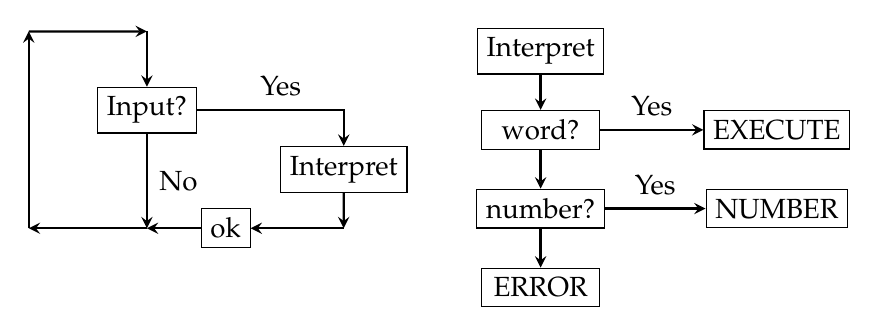
\begin{tikzpicture}[node distance=2cm]
            %Create nodes for left loop
            \node (input_1)     [wordinr1] {Input?}    ;
            \node (interpret_1) [wordinr1, right of = input_1, xshift=0.5cm, yshift=-0.75cm] {Interpret};
            \node (ok)          [wordinr1, below of = input_1, xshift=1.0cm, yshift=0.5cm] {ok};
            \coordinate[below of=input_1, yshift=0.5cm] (cont_1);
            \coordinate[left  of=cont_1,  xshift=0.5cm] (cont_2);
            \coordinate[above of=cont_2, yshift=0.5cm] (cont_3);
            \coordinate[above of=input_1, yshift=-1.0cm] (cont_4);
            \coordinate[below of=input_1, xshift=2.5cm, yshift=0.5cm] (cont_5);
            %Connect left loop
            \draw [arrow] (input_1.south) -- node[xshift=0.40cm] {No} (cont_1.north);
            \draw [arrow] (ok.west)       -- (cont_1.east);
            \draw [arrow] (cont_1.west)   -- (cont_2.east);
            \draw [arrow] (cont_2.north)  -- (cont_3.south);
            \draw [arrow] (cont_3.east)   -- (cont_4.west);
            \draw [arrow] (cont_4.south)  -- (input_1.north);
            %Connect right loop
            \draw [arrow] (input_1.east)  -| node[yshift=0.30cm, xshift=-0.80cm] {Yes} (interpret_1.north) ;
            \draw [arrow] (interpret_1.south) -- (cont_5.north);
            \draw [arrow] (cont_5.west) -- (ok.east) ;
            
            \node (interpret_2) [wordinr2, yshift=0.75cm, xshift=5.0cm]           {Interpret} ;
            \node (word)        [wordinr2, yshift=1.0cm,  below of = interpret_2] {word?}     ;
            \node (number_1)    [wordinr2, yshift=1.0cm,  below of = word, ]      {number?}   ;
            \node (error)       [wordinr2, yshift=1.0cm,  below of = number_1]    {ERROR}     ;
            \node (execute)     [wordinr2, xshift=1.0cm,  right of = word]        {EXECUTE}   ;
            \node (number_2)    [wordinr2, xshift=1.0cm,  right of = number_1]    {NUMBER}    ;
            \draw [arrow] (interpret_2) -- (word);
            \draw [arrow] (word)        -- (number_1);
            \draw [arrow] (number_1)    -- (error);
            \draw [arrow] (word)        -- node[yshift=0.30cm] {Yes} (execute);
            \draw [arrow] (number_1)    -- node[yshift=0.30cm] {Yes} (number_2);
        \end{tikzpicture}
    }
  \caption{\textit{Overview of FORTH outer interpreter}}
  \label{fig:Outer_interpreter}
\end{figure}

In general, because FORTH is interpretive as well as compiled, the best way to study something new is in front of a computer running FORTH. Therefore we explain with illustrations, expecting the reader to try them out.

In what follows, anything the user types in will be set in \lstinline$Helvetica$, such as \regc{DECIMAL} below.

Machine responses appear in ordinary type.

We now give a trivial illustration:

\begin{lstlisting}
DECIMAL <cr> ok
\end{lstlisting}

\underline{\textbf{Notes}}:
\begin{itemize}
  \item \bc{<cr>} means "the user pushes the ENTER or $\Leftarrow$ button".
  \item \bc{ok} is what FORTH says in response to an input line, if nothing has gone wrong.
  \item \regc{DECIMAL} is an instruction to use base 10 arithmetic. FORTH will use any base on tell it, within reason, but usually only \regc{DECIMAL} and \regc{HEX} (hexadecimal) are predefined.
\end{itemize}

When the outer interpreter (see fig. 2.1 on p. 13) encounters text with no dictionary entry, it tries to interpret it as a \bc{NUMBER}.

It places the number in a special memory location called "the top of the stack" (TOS)\footnote{We will explain about the stack in §2.3.}
\begin{lstlisting}
2 17 +. <cr> 19 ok
\end{lstlisting}

\underline{\textbf{Notes}}:
\begin{itemize}
  \item FORTH interprets 2 and 17 as numbers, and pushes them onto the stack. "\bc{+}" is a word and so is "\bc{.}" so they are \bc{EXECUTE}d.
  \item \lstinline$+$ adds 2 to 17 and leaves 19 on the stack.
  \item The word \bc{.} (called "emit") removes 19 from the stack and displays it on the screen.
\end{itemize}

We might also have said \footnote{since FORTH uses words, when we enter an input line we say the corresponding phrase.}

\begin{lstlisting}
HEX 0A 14 * . <cr> C8 ok
\end{lstlisting}

(Do you understand this? Hint: \bc{HEX} stands for "switch to hexadecimal arithmetic")

If the incoming text can neither be located in the dictionary nor interpreted as a number, FORTH issues an error message.


\section{Extending the dictionary}

\TallC{T}{he} compiler is one of FORTl-I’s most endearing features. It is elegant, simple, and mostly written in FORTH. Although the technical details of the FORTH compiler are generally more interesting to systems developers than to scientists, its components can often be used to solve programming problems. When this is the case, we necessarily discuss details of the compiler. In this section we discuss how the compiler extends the dictionary. In §2§§8 below we examine the parts of the compiler in greater detail.

FORTH has special words that allow the creation of new dictionary entries, \textit{i.e.}, new words. The most important are "\bc{:}" ("start a new definition") and "\bc{;}" ("end the new definition").

Consider the phrase

\begin{lstlisting}
: NEW-WORD WORD1 17 WORDZ . . . WORDn ; ok
\end{lstlisting}

The initial "\bc{:}" is \bc{EXECUTE}d because it is already in the dictionary. Upon execution, "\bc{:}" does the following:

\begin{itemize}
    \item Creates a new dictionary entry, \bc{NEW-WORD}, and switches from \textbf{interpret}- to \textbf{compile} mode.
    \item In compile mode, the interpreter looks up words and — rather than executin them — installs ointers to their code. If the text is a number (\bc{17} above), FORTH builds the literal number into the dictionary space allotted for \bc{NEW-WORD}.
    \item The action of \bc{NEW-WORD} will be to \bc{EXECUTE} sequentially the previously-defined words \bc{WORD1}, \bc{WORD2}, ...\bc{WORDn}, placing any built-in numbers on the stack as they occur.
    \item The FORTH compiler \bc{EXECUTE}s the last word "\bc{;}" of the definition, by installing code (to return control to the next outer level of the interpreter\footnote{This level could be either the outer interpreter or a word that invokes \bc{NEW-WORD}.}) then switching back from compile to interpret mode. Most other languages treat tokens like "\bc{;}" as flags (in the input stream) that \textit{trigger} actions, rather than actions in their own right FORTH lets components execute themselves.
\end{itemize}

In FORTH \textit{all} subroutines are words that are invoked when they are named. No explicit CALL or GOSUB statement is required.

The above definition of \textbf{NEW-WORD} is extremely structured compared with FORTRAN or BASIC. Its definition is just a series of subroutine calls.

\TallC{W}{e} now illustrate how to define and use a new word using the previously defined words "\bc{:}"and "\bc{;}". Enter the phrase (this new word \bc{*+} expects 3 numbers, \textit{a}, \textit{b}, and \textit{c} on the stack)

\begin{lstlisting}
: *+   * + ; ok
\end{lstlisting}

\underline{Notes:}
\begin{itemize}
    \item \bc{*} multiplies b with c, leaving b*c.
    \item \bc{+} then adds b*c to a, leaving a + b*c behind.
\end{itemize}

Now we actually try out \bc{*+} :

\begin{lstlisting}
DECIMAL 5 6 7 *+ . 47 ok
\end{lstlisting}

\underline{\textbf{Notes:}}
\begin{itemize}
    \item The period \bc{.} is not a typo, it EMlTs the result.
    \item FORTH's response to \bc{a b c *+ .} is \bc{a + b*c ok}.
\end{itemize}

What if we were to enter *+ with nothing on the stack? Let's try it and see (\bc{.S} is a word that displays the stack without changing its contents):

\begin{lstlisting}
.S empty stack ok

*+ empty stack ok
\end{lstlisting}

\dotrule{1\textwidth}

\underline{\textbf{Exercise:}}

Suppose you entered the input line

\begin{lstlisting}
HEX 5 6 7 *+ . <cr> xxx ok
\end{lstlisting}

What would you expect the response \textbf{xxx} to be?

\textit{Answer:} \bc{2F}

\dotrule{1\textwidth}

\section{Stacks and reverse Polish notation (RPN)}

\TallC{W}{e} now discuss the stack and the "reverse Polish" or "postfix" arithmetic based on it. (Anyone who has used one of the Hewlett-Packard calculators should already be familiar with the basic concepts.)

A Polish mathematician (J .Lukasewcleia) showed that numerical calculations require an irreducible minimum of elementary operations (fetching and storing numbers as well as addition, subtraction, multiplication and division). The minimum is obtained when the calculation is organized by "stack" arithmetic.

Thus virtually all central processors (CPU's) intended for arithmetic operations are designed around stacks. FORTH makes efficient use of CPU's by reflecting this underlying stack architecture in its syntax, rather than translating algebraic-looking program statements ("infix" notation) into RPN-based machine operations as FORTRAN, BASIC, C and Pascal do.

But what \textit{is} a stack? As the name implies, a stack is the machine analog of a pile of cards with numbers written on them. Numbers are always added to, and removed from, the top of the pile. (That is, a stack resembles a job where layoffs follow seniority: last in, first out.) Thus, the FORTH input line

\begin{lstlisting}
DECIMAL 2 5 73 -16 ok
\end{lstlisting}

followed by the line

\begin{lstlisting}
+ - * . yyy ok
\end{lstlisting}

leaves the stack in the successive states shown in Table 2-1 below

\begin{center}
    \begin{tabular}{|c c c c c c c|}
        \hline
   Cell\# & Initial    & Ops$\rightarrow$ & +       & -          & *       & . \\ [0.5ex] 
        \hline
        0 & \lgray -16 & Result        & \Aggray 57 & \dgray -52 & \gray 104 & ... \\ 
        1 & \lgray 73  & $\rightarrow$ & \Aggray 5  & \dgray 2   & ...       & ... \\
        2 & \lgray 5   &               & \Aggray 2  & ...        & ...       & ... \\
        3 & \lgray 2   &               & ...        & ...        & ...       & ... \\
        \hline
    \end{tabular}
\end{center}

Table 2-1 \textit{Picture of the stack during operations}

We usually employ zero-based relative numbering in FORTH data structures —stacks, arrays, tables, \textit{etc}.— so TOS ("top of stack") is given relative \#0, NOS ("next on stack") \#1, \textit{\textit{etc}}.

The operation "\bc{.}" ("emit") displays -104 to the screen, leaving the stack empty. That is, \bc{yyy} above is \bc{-104}.

\subsection{Manipulating the parameter stack}

\TallC{F}{ORTH} system incorporate (at least) two stacks: the \textbf{parameter} stack which we now discuss, and the \textbf{return stack} which we defer to 2.3.2.

In order to use a stack-based system, we must be able to put numbers on the stack, remove them, and rearrange their order. FORTH includes standard words for this purpose.

Putting numbers on the stack is easy: one simply types the number (or it appears in the definition of a FORTH word).

To remove a number we have the word \bc{DROP} that drops the number from TOS and moves up all the other numbers.

Tb exchange the top 2 numbers we have .

\bc{DUP} duplicates the TOS into NOS, pushing down all the other numbers.

\bc{ROT} rotates the top 3 numbers.

\begin{center}
    \begin{tabular}{|c c c c c c c|}
        \hline
   Cell\# & Initial    & Ops$\rightarrow$ & DROP   & SWAP        & ROT       & DUP\\ [0.5ex] 
        \hline
        0 & \lgray -16 & Result        & \Aggray 73 & \dgray 73  & \gray 5   & \digray -16 \\ 
        1 & \lgray 73  & $\rightarrow$ & \Aggray 5  & \dgray -16 & \gray -16 & \digray -16 \\
        2 & \lgray 5   &               & \Aggray 2  & \dgray 5   & \gray 73  & \digray 73  \\
        3 & \lgray 2   &               & ...        & \dgray 2   & \gray 2   & \digray 5   \\
        4 & \lgray ... &               & ...        & ...        & ...       & \digray 2   \\
        \hline
    \end{tabular}
\end{center}

Table 2-2 \textit{Stack manipulation operators}

These actions are shown on page 19 above in Thble 2—2 (we show what each word does to the initial stack).

In addition the words \bc{OVER}, \bc{UNDER}, \bc{PICK} and \bc{ROLL} act as shown in Table 2-3 below (note \bc{PICK} and \bc{ROLL} must be preceded by an integer that says where on the stack an element gets  \bc{PICK}ed or \bc{ROLL}ed).

\begin{center}
    \begin{tabular}{|c c c c c c c|}
        \hline
   Cell\# & Initial    & Ops$\rightarrow$ & OVER   & UNDER        & 4 PICK  & 4 ROLL \\ [0.5ex] 
        \hline
        0 & \lgray -16 & Result        & \Aggray 73  & \dgray -16 & \gray 2   & \digray 2   \\ 
        1 & \lgray 73  & $\rightarrow$ & \Aggray -16 & \dgray 73  & \gray -16 & \digray -16 \\
        2 & \lgray 5   &               & \Aggray 73  & \dgray -16 & \gray 73  & \digray 73  \\
        3 & \lgray 2   &               & \Aggray 5   & \dgray 5   & \gray 5   & \digray 5   \\
        4 & \lgray ... &               & \Aggray 2   & \dgray 2   & \gray 2   & ...         \\
        \hline
    \end{tabular}
\end{center}

Table 2-3 \textit{More stack manipulation operators}

Clearly, \bc{1 PICK} is the same as \bc{DUP}, \bc{2 PICK} is a synonym for \bc{OVER}, \bc{2 ROLL} means \bc{SWAP}, and \bc{3 ROLL} means \bc{ROT}.

As Brodie has noted (\TF), it is rarely advisable to have aword use a stack so deep that \bc{PICK} or \bc{ROLL} is needed. It is generally better to keep word definitions short, using only a small number of arguments on the stack and consuming them to the extent possible. On the other hand, \bc{ROT} and its opposite, \bc{-ROT}\footnote{defined as \bc{: -ROT ROT ROT ;}}, are often useful.

\subsection{The return stack and Its uses}
\TallC{W}{e} have remarked above in §2§§2 that compilation establishes links from the calling word to the previously- defined word being invoked. Part of the linkage mechanism ——during actual execution- is the \textbf{return stack} (rstack): the address of the next word to be invoked after the currently executing word is placed on the rstack, so that when the current word is done, the system jumps to the next word. Although it might seem logical to call the address on the rstack the \textbf{next} address, it is actually called the \textbf{return} address for historical reasons.

In addition to serving as a reservoir of return addresses (since words can be nested, the return addresses need a stack to be put on) the rstack is where the limits of a \bc{DO ... LOOP} construct are placed\footnote{We discuss looping in 2.7 below.}

The user can also store/retrieve to/from the rstack This is an example of using a component for a purpose other than the one it was designed for. Such use is not encouraged by every FORTH text, needless to say, since it introduces the spice of danger. To store to the rstack we say \bc{>R}, and to retrieve we say \bc{R>}. \bc{DUP>R} is a speedup of the phrase \bc{DUP >R}. The words \bc{D>R DR>} , for maving double-length integers, also exist on many systems. The word \bc{R@} copies the top of the rstack to the TOS.

\leftbar[1\linewidth]
\textbf{The danger is this:} anything put on the rstack during a word’s execution must be removed before the word terminates. If the \bc{>R} and the \bc{R>} do not balance, then a \textbf{wrong next address} will be jumped to and \bc{EXECUTE}d. Since this could be the address of data, and since it is being interpreted as machine instructions, the results will be \textbf{always unpredictable}, but seldom amusing.
\endleftbar

Why would we want to use the rstack for storage when we have a perfectly good parameter stack to play with? Sometimes it becomes simply impossible to read code that performs complex gymnastics on the parameter stack, even though FORTH permits such gymnastics.

Consider a problem — say, drawing a line on a bit- mapped graphics output device from (x,y) to (x',y')— that requires 4 arguments. We have to turn on the appropriate pixels in the memory area representing the display, in the ranges from the origin to the end coordinates of the line. Suppose we want to work with x and y first, but they are 3rd and 4th on the stack. So we have to \bc{ROLL} or \bc{PICK} to get them to TOS where they can be worked with conveniently. We probably need them again, so we use

\begin{lstlisting}
4PICK 4PICK ( -- x y x' y' x y)
\end{lstlisting}

Now 6 arguments are on the stack! See what I mean? A better way stores temporarily the arguments x’ and y', leaving only 2 on the stack. If we need to duplicate them, we can do it with an already existing word, \bc{DDUP}.

Complex stack manipulations can be avoided by defining \bc{VARIABLE}s —named locations— to store numbers. Since FORTH, variables are typically \textit{global} —any word can access them — their use can lead to unfortunate and unexpected interactions among parts of a large program. Variables should be used sparingly.

While FORTH permits us to make variables local to the sub- if routines that use them\footnote{See \FTR, p. 3253 for a description of beheading - a process to make variables local to a small set of subroutines. Another technique is to embed variables within a data structure so they cannot be referenccd inadvertently. Chapters 2§8§§3-2, 3§5§§2, 5§1§§2 and 11§2 offer examples.}, for many purposes the rstack can advantageously replace local variables:

\begin{itemize}
    \item The rstack already exists, so it need not be defined anew.
    \item When the numbers placed on it are removed, the rstack shrinks, thereby reclaiming some memory.
\end{itemize}

Suppose, in the previous example, we had put x’ and y’ on the rstack via the phrase

\begin{lstlisting}
    >R >R DDUP .
\end{lstlisting}

Then we could duplicate and access x and y with no trouble.

\leftbar[1\linewidth]
\underline{\textbf{A note of caution}}: since the rstack is a critical component of the execution mechanism, we mess with it at our peril. If we want to use it, we must clean up when we are done, so it is in the same state as when we found it. A word that places a number on the rstack must get it off again — using \bc{R>} or \bc{RDROP} — before exiting that word\footnote{\textbf{RDROP} is a handy way to exit from a word before reaching the final ";". See \TF.}. Similarly, since no LOOP uses the rstack also, for each >R in such a loop (after DO) there must be a corresponding R > or RDROP (before LOOP is reached). Otherwise the results will be unpredictable and probably will crash the system.
\endleftbar

\section{Fetching and storing}

\TallC{O}{rdinary} (16-bit) numbers are f\textit{etc}hed from memory to the stack by "\bc{@}" ("fetch"), and stored by "\bc{!}" ("store"). The word @ expects an address on the stack and replaces that address by its contents using, \textit{e.g.}, the phrase \bc{X @}. The word "\regc{!}" expects a number (NOS) and an address (T OS) to store it in, and places the number in the memory location referred to by the address, consuming both arguments in the process, as in the phrase \bc{32 X !}

Double length (32-bit) numbers can similarly be f\textit{etc}hed and stored, by \bc{D@} and \bc{DI} . (FORTH systems designed for the newer 32-bit machines sometimes use a 32-bit-wide stack and may not distinguish between single- and double-length integers.)

Positive numbers smaller than 255 can be placed in single bytes of memory using \bc{C@} and \bc{C!}. This is convenient for operations with strings of ASCII text, for example screen, file and keyboard I/O.

In Chapters 3, 4, S and 7 we shall extend the lexicon of \regc{@} and \regc{!} words to include floating point and complex numbers.

\section{Arlthmetlc operations}

\TallC{T}{he} 1979 or 1983 standards, not to mention the forthcoming ANSII standard, require that a conforming FORTH system contain a certain minimum set of predefined words. These consist of arithmetic operators \bc{+ — * / MOD /MOD */} for (usually) 16-bit \textit{signed-integer} (-32767 to +32767) arithmetic, and equivalents for \textit{unsigned} (0 to 65535), double-length and mixed-mode (16- mixed with 32-bit) arithmetic. The list will be found in the glossary accompanying your system, as well as in \SF and \FTR.

\section{Comparing and testlng}

TallC{I}{n} addition to arithmetic, FORTH lets us compare numbers on the stack, using relational operators \bc{> < =}.These operators work as follows: the phrase

\begin{lstlisting}
    2 3 > < cr > ok
\end{lstlisting}

will leave 0 ("false") on the stack, because 2 (N0S) is not greater
than 3 (TOS). Conversely, the phrase

\begin{lstlisting}
    23 < <cr> ok
\end{lstlisting}

will leave -1 ("true") because 2 is less than 3. Relational operators typically consume their arguments and leave a "flag" to show what happened\footnote{The original FORTH-79 used +1 for "true", 0 for "false"; many newer system that mostly follow FORTH-79 use -1 for "true". HS/FORTH is one such. Both FORTH-83 and ANSII FORTH require -1 for "true", 0 for "false".}. Those listed so far work with signed 16-bit integers. The operator \bc{U<} tests \textit{unsigned} 16-bit integers (0-65535).

FORTH offers unary relational operators \bc{0= 0>} and \bc{0<} that determine whether the TOS contains a (signed) 16-bit integer that is 0, positive or negative. Most FORTHs offer equivalent relational operators for use with double-length integers.

The relational words are used for branching and control. The usual form is

\begin{lstlisting}
    : MAYBE 0> IF WORDl WORD2 ...
      WORDn THEN ;
\end{lstlisting}

The word \bc{MAYBE} expects a number on the stack, and executes the words between \bc{IF} and \bc{THEN} if the number on the stack is positive, but not otherwise. If the number initially on the stack were negative or zero, \bc{MAYBE} would do nothing.

An alternate form including \bc{ELSE} allows two mutually exclusive actions:

\begin{lstlisting}
    : CHOOSE 0> IF WORD1 . . . WORDn
            ELSE WORDt' . . . WORDn'
            THEN ; (n -- )
\end{lstlisting}

If the number on the stack is positive, \bc{CHOOSE} executes \bc{WORD1 WORD2... WORD}, whereas if the number is negative or 0, \bc{CHOOSE} executes \bc{WORD1'} ... \bc{WORDn'}.

In either example, \bc{THEN} marks the end of the branch, rather than having its usual logical meaning\footnote{This has led some FORTH gurus to prefer the synonymous word \bc{ENDIF} as clearer than \bc{THEN}.}.

\section{Looping and structured programming}

\TallC{F}{ORTH} contains words for setting up loops that can be definite or indefinite:

\begin{lstlisting}
    BEGIN xxx flag UNTIL
\end{lstlisting}

The words represented by \bc{xxx} are executed, leaving the TOS (flag) set to 0 (F) -at which point \bc{UNTIL} leaves the loop - or -1 (T) -at which point \bc{UNTIL} makes the loop repeat from \bc{BEGIN}.

A variant is
\begin{lstlisting}
    BEGIN xxx flag WHILE yyy REPEAT
\end{lstlisting}

Here \bc{xxx} is executed, \bc{WHILE} tests the flag and if it is 0 (F) leaves the loop; whereas if flag is -1 (T) \bc{WHILE} executes \bc{yyy} and \bc{REPEAT} then branches back to \bc{BEGIN}. These forms can be used to set up loops that repeat until some external event (pressing a key at the keyboard, \textit{e.g.}) sets the flag to exit the loop. They can also used to make endless loops (like the outer interpreter of FORTH) by forcing flag to be 0 in a definition like

\begin{lstlisting}
    : ENDLESS BEGIN xxx 0 UNTIL ;
\end{lstlisting}

\TallC{F}{ORTH} also implements indexed loops using the words \bc{DO LOOP +LOOP /LOOP}. These appear within definitions, \textit{e.g.}

\begin{lstlisting}
    : LOOP-EXAMPLE 100 0 DO xxx LOOP ;
\end{lstlisting}

The words \bc{xxx} will be executed 100 times as the lower limit, 0, increases in unit steps to 99. To step by -2's, we use the phrase

\begin{lstlisting}
    -2 + LOOP
\end{lstlisting}

to replace \bc{LOOP}, as in

\begin{lstlisting}
    : DOWN-BY-2's O 100 DO xxx -2 +LOOP ;
\end{lstlisting}

The word \bc{/LOOP} 1s a variant of \bc{+LOOP} for working with unsigned limits\footnote{Signed 16-bit integers run from -32768 to +32767, unsigned from 0 to 65535. See \FTR.} and increments (to permit the loop index to go up to 65535 in 16-bit systems).

\section{The pearl of FORTH}

An unusual construct, \bc{CREATE...DOES>}, has been called "the pearl of FORTH" \footnote{Michael Ham, "Structured Programming", \textit{Dr. Dobb's Journal of Software Tools}, October, 1986.} This is more than poetic license.

\bc{CREATE} is a component of the compiler that makes a new dictionary entry with a given name (the next name in the input stream) and has no other function.

\bc{DOES>} assigns a specific run-time action to a newly \bc{CREATE}d word (we shall see this in §2§§8-3 below).

\subsection{Dummy words}
Sometimes we use \bc{CREATE} to make a dummy entry that we can later assign to some action:
\begin{lstlisting}
    CREATE DUMMY
    CA' * DefinES DUMMY
\end{lstlisting}

The second line translates as "The code address of \bc{*} defines \bc{DUMMY}". Entry of the above phrase would let \bc{DUMMY} perform the job of \bc{*} just by saying \bc{DUMMY}. That is, FORTH lets us first define a dummy word, and then give it any other word’s meaning \footnote{This usage is a non-standard construct of HS/FORTH.}.

Here is one use of this power: Suppose we have to define two words that are alike except for some piece in the middle:
\begin{lstlisting}
    : *WORD  WORD1 WORD2 *  WORD3 WORD4 ;
    : */WORD WORD1 WORD2 */ WORD3 WORD4 ;
\end{lstlisting}

we could get away with 1 word, together with \bc{DUMMY} fromabove,

\begin{lstlisting}
    : *_or_*/WORD
        WORD1 WORD2
        DUMMY
        WORD3 WORD4 ;
\end{lstlisting}
by saying
\begin{lstlisting}
    CA' * DefinES DUMMY *_or_*/WORD
\end{lstlisting}
or
\begin{lstlisting}
    CA' */ DefinES DUMMY *_or_*/WORD
\end{lstlisting}

This technique, a rudimentary example of vectoring, saves memory and saves programming time by letting us vary something in the middle of a definition \textit{after the definition has been entered in the dictionary}. However, this technique must be used with caution as it is akin to \textbf{self-modifying} code\footnote{Self-modifying machine code is considered a serious "no-no" by modern structured programming standards. Although it is sometimes valuable, few modern cpu's are capable of handling it safely. More often, because cpu's tend to use pipelining and parallelism to achieve speed, a piece of code might be modified in memory, but - having been pre-fetched before modification - actually execute in unmodified form.}

A similar procedure lets a subroutine call itself recursively, an enormous help in coding certain algorithms.

\subsection{Defining "defining" words}

\TallC{T}{he} title of this section is neither a typo nor a stutter: \bc{CREATE} finds its most important use in extending the powerful class of FORTH words called "defining" words. The colon compiler "\bc{:}" is such a word, as are \bc{VARIABLE} and \bc{CONSTANT}. The definition of \bc{VARIABLE} is simple

\begin{lstlisting}
    : VARIABLE CREATE 2 ALLOT ;
\end{lstlisting}

Here is how we use it:
\begin{lstlisting}
    VARIABLE X <cr> ok
\end{lstlisting}

The inner workings of VARIABLE are these:
\begin{itemize}
    \item \bc{CREATE} makes a dictionary entry with the next name in the input stream — in this case, \bc{X}.
    \item Then the number 2 is placed on the stack, and the word \bc{ALLOT} increments the pointer that represents the current location in the dictionary by 2 bytes.
    \item This leaves a 2-byte vacancy to store the value of the variable (that is, the next dictionary header begins 2 bytes above the end of the one just defined).
\end{itemize}

When the outer interpreter loop encounters a new \bc{VARIABLE}'s name in the input stream, that name’s address is placed on the stack. But this is also the location where the 2 bytes of storage begins. Hence when we type in \bc{X}, the TOS will contain the storage address named \bc{X}.

As noted in §2.4 above, the phrase \bc{X @} (pronounced "X f\textit{etc}h") places the contents of address \bc{X} on the stack, dropping the address in the process. Conversely, to store a value in the named location \bc{X}, we use \bc{!} ("store"): thus
\begin{lstlisting}
    4 X ! <cr> ok
    X @ . <cr> 4 ok
\end{lstlisting}

Double-length variables are defined \textit{via} \bc{DVARIABLE}, whose definition is

\begin{lstlisting}
    : DVARIABLE CREATE 4 ALLOT ;
\end{lstlisting}

\TallC{F}{ORTH} has a method for defining words initialized to contain specific values: for example, we might want to define the number 17 to be a word. \bc{CREATE} and "\bc{,}" ("comma") let us do this as follows:

\begin{lstlisting}
    17 CREATE SEVENTEEN , <cr> ok
\end{lstlisting}

Now test it \textit{via}

\begin{lstlisting}
    SEVENTEEN @ . <cr> 17 ok
\end{lstlisting}

\underline{\textbf{Note}}: The word "," ("comma") puts TOS into the next 2 bytes of the dictionary and increments the dictionary pointer by 2.

A word \bc{C}, ("see-comma") puts a byte-value into the next byte of the dictionary and increments the pointer by 1 byte.

\subsection{Run-time vs. compile-time actions}

\TallC{I}{n} the preceding example, we were able to initialize the variable \bc{SEVENTEEN} to 17 when we \bc{CREATE}d it, but we still have to fetch it to the stack \textit{via} \bc{SEVENTEEN @} whenever we want it. This is not quite what we had in mind: we would like to find 17 in T0S when we say \bc{SEVENTEEN}. The word \bc{DOES>} gives us precisely the tool to do this.

As noted above, the function of \bc{DOES>} is to specify a run-time action for the "child" words of a defining word. Consider the defining word \bc{CONSTANT}, defined in high-level\footnote{Of course \bc{CONSTANT} is usually a machine—code primitive, for speed.} FORTH by

\begin{lstlisting}
    : CONSTANT CREATE , DOES> @ ;
\end{lstlisting}
and used as
\begin{lstlisting}
    53 CONSTANT PRIME ok
\end{lstlisting}

Now test it:
\begin{lstlisting}
    \textbf{PRIME} . <cr> 53 ok
\end{lstlisting}

What happened?
\begin{itemize}
    \item \bc{CREATE} (hidden in \bc{CONSTANT}) made an entry (named \bc{PRIME} , the first word in the input stream following \bc{CONSTANT}). Then "\bc{,}" placed the TOS (the number 53) in the next two bytes of the dictionary.
    \item \bc{DOES>} (inside \bc{CONSTANT}) then appended the actions of all words between it and "\bc{;}" (the end of the definition of \bc{CONSTANT}) to the child word(s) defined by \bc{CONSTANT}.
    \item In this case, the only word between \bc{DOES>} and \bc{;} was \bc{@} , so all FORTH constants defined by CONSTANT perform the action of placing their address on the stack (anything made by \bc{CREATE} does this) and fetching the contents of this address.
\end{itemize}

\subsubsection{Klingons}

\TallC{L}{et} us make a more complex example. Suppose we had previously defined a word \bc{BOX ( n x y -- )} that draws a small square box of n pixels to a side centered at (x, y) on the graphics display. We could use this to indicate the instantaneous location of a moving object -- say a Klingon space-ship in a space-war game.

So we define a defining word that creates (not very realistic looking) space ships as squares n pixels on a side:

\begin{lstlisting}
    : SPACE-SHIP CREATE , DOES>
        @-ROT (--nxy)      BOX ;
    : SIZE ; \ do-nothing word
\end{lstlisting}

Now, the usage would be (\bc{SIZE} is included merely as a reminder of what 5 means -- it has no function other than to make the definition look like an English phrase)

\begin{lstlisting}
    SIZE 5 SPACE-SHIP KLINGON <cr> ok
    71 35 KLINGON <cr> ok
\end{lstlisting}

Of course, \bc{SPACE-SHIP} is a poorly constructed defining word because it does not do what it is intended to do. Its child-word \bc{KLINGON} simply draws itself at (x, y).

What we really want is for \bc{KLINGON} to \textit{undraw} itself from its old location, compute its new position according to a set of rules, and then redraw itself at its new position This sequence of operations would require a definition more like

\begin{lstlisting}
    :OLD.POS@ (adr--adr n x y) DUP @ OVER
      2+ D@ :
    : SPACE-SHIP CREATE , 4 ALLOT DOES>
       OLD.POS@ UNBOX NEW.POSI
       OLD.POS@ BOX DROP ;
\end{lstlisting}

where the needed specialized operation \bc{UNBOX} would be defined previously along with \bc{BOX}.

\subsubsection{Dimensioned data (with Intrinsic unlts)}
Here is another example of the power of defining words and of the distinction between compile-time and run-time behaviors.

Physical problems generally work with quantities that have dimensions, usually expressed as mass (M), length (L) and time (T) or products of powers of these. Sometimes there is more than one system of units in common use to describe the same phenomena.

For example, traffic police reporting accidents in the United States or the United Kingdom might use inches, feet, and yards; whereas Continental police would use the metric system. Rather than write different versions of an accident analysis program it is simpler to write one program and make unit conversions part of the grammar. This is easy in FORTH; impossible in FORTRAN, BASIC, Pascal, or C; and possible, but exceedingly cumbersomein Ada\footnote{An example (and its justification) of dimensioned data types in Ada is given by Do-While Jones, \textit{Dr. Dobb's Journal}, March 1987. The FORTH solution below is much simpler than the Ada version.}.

We simply keep all internal lengths in millimeters, say, and con-
vert as follows\footnote{This example is based on 16-bit integer arithmetic. The word \regc{*/} means "multiply the third number on the stack by NOS, keeping 32 bits of precision, and divide by "TOS". That is, the stack comment for \regc{*/} is \regc{(a b c --a*b/c)}.}:

\begin{lstlisting}
    : INCHES  254 10 */ ;
    : FEET  [ 254 12 * ] LITERAL 10 */ ;
    : YARDS [ 254 36 * ] LITERAL 10 */ ;
    : CENTIMETERS 10 * ;
    : METERS 1000 * ;
\end{lstlisting}

The usage would be
\begin{lstlisting}
    10 FEET . <cr> 3048 ok
\end{lstlisting}

These are more definitions than necessary, of course, and the technique generates unnecessary code. A more compact approach uses a \textit{defining word}, \bc{UNITS}:

\begin{lstlisting}
    : D, SWAP , , ; \ I double—length # in next cells
    : UNITS CREATE D, DOES> D@ */ ;
\end{lstlisting}

Then we could make the table
\begin{lstlisting}
    254  10         UNITS INCHES
    254  12 * 10    UNITS FEET
    254  36 * 10    UNITS YARDS
     10   1         UNITS CENTIMETERS
    1000  1         UNITS METERS
    \ Usage:
    \ 10 FEET . <cr> 3048 ok
    \ 3  METERS . <cr> 3000 ok
    \ ......
    \ \textit{etc}.
\end{lstlisting}

This is an improvement, but FORTH lets us do even better: here is a simple extension that allows conversion back to the input units, for use in output:

\begin{lstlisting}
    VARIABLE <AS>                \ new variable
    0 <AS> !                     \ initialize to "F"
    : AS -1 <AS> ! ;             \ set <AS> = "T"
    : UNITS CREATE D, DOES>
       D@                        \ get 2 #s
       <AS> @                    \ get current val.
          IF SWAP THEN           \ flip if "true"
      */   0 <AS> ! ;            \ convert, reset <AS>

    BEHEAD' <AS>          \ make it local for security(*@\footnote{Headerless words are described in \FTR, p. 325ff. The word \textbf{BEHEAD'} is HS/FORTH's method for making a normal word into a headerless one. See Ch. 5\S1\S\S3 for further details.} @*)
    \ unit definitions remain the same
    \ Usage:
    \ 10 FEET      . <cr> 3048 ok
    \ 3048 AS FEET . <cr> 10 ok
\end{lstlisting}

\subsection{Advanced methods of controlllng the compiler}

\TallC{F}){ORTH} includes a technique for switching from compile mode to interpret mode while compiling or interpreting. This is done using the words \bc{]} and \bc{[} . (Contrary to intuition, \bc{]} turns the compiler on, \bc{[} turns it off.)

One use of \bc{]} and \bc{[} is to create an "action table" that allows us to choose which of several actions we would like to perform\footnote{Better methods will be described in Chapter 5.}.

For example, suppose we have a series of push-buttons numbered 1-6, and a word \bc{WHAT} to read them.

That is, \bc{WHAT} waits for input from a keypad; when button \#3 is pushed, \textit{e.g.}, \bc{WHAT} leaves 3 on the stack.

We would like to use the word \bc{BUTTON} in the following way:

\begin{lstlisting}
    WHAT BUTTON
\end{lstlisting}

\bc{BUTTON} can be defined to choose its action from a table of
actions called \bc{BUTTONS} . We define the words as follows:

\begin{lstlisting}
    CREATE BUTTONS ] RING-BELL OPEN-DOOR
      ENTER LAUGH CRY SELF-DESTRUCT [
    : BUTTON 1- 2* BUTTONS + @ EXECUTE ;
\end{lstlisting}

If, as before, I push \#3, then the action \bc{ENTER} will be executed. Presumably button \#7 is a good one to avoid\footnote{The safety of an execution table can be increased by making the first (that is, the zero’th) action \textbf{WARNING}, and making the first step of \bc{BUTTON} a word \bc{CHECK-DATA} that maps any number not in the range 1-6 into 0. Then a wrong button number causes a \textbf{WARNING} to be issued and the system resets.}.

How does this work?
\begin{itemize}
    \item \bc{CREATE BUTTONS} makes a dictionary entry \bc{BUTTONS}.
    \item \bc{]} turns on the compiler: the previously-defined word-names \bc{RING-BELL}, \textit{etc.} are looked up in the dictionary and compiled into the table (as though we had begun with :), rather than being executed.
    \item \bc{[} returns to interactive mode (as if it were ;), so that the next colon definition (\bc{BUTTON}) can be processed.
    \item The table \bc{BUTTONS} now contains the code-field addresses (CFA’s) of the desired actions of \bc{BUTTON}.
    \item \bc{BUTTON} first uses 1- to subtract 1 from the button number left on the stack by \bc{WHAT} (so we can use 0—based numbering into the table -- if the first button were \# 0, this would be unneeded).
    \item \bc{2*} then multiplies by 2 to get the offset (from the beginning of \bc{BUTTONS}) of the CFA representing the desired action.
    \item \bc{BUTTONS +} then adds the base address of \bc{BUTTONS} to get the absolute address where the desired CPA is stored.
    \item \bc{@} fetches the CFA for \bc{EXECUTE} to execute.
    \item \bc{EXECUTE} executes the word corresponding to the button pushed. Simple!
\end{itemize}

You may well ask "Why bother with all this indirection, pointers, pointers to pointers, tables of pointers to tables of pointers, and the like?" Why not just have nested \bc{IF...ELSE...THEN} constructs, as in Pascal?

There are three excellent reasons for using pointers:
\begin{itemize}
    \item Nested \bc{IF...THEN}'s uickly become cumbersome and difficult to decipher (\TF). They are also \underline{\textbf{slow}} (see Ch. 11).
    \item Changing pointers is generally much faster than changing other kinds of data -- for example reading in code overlays to accomplish a similar task.
    \item The unlimited depth of indirection possible in FORTH permits arbitrary levels of abstraction. This makes the computer behave more "intelligently" than might be possible with more restrictive languages.
\end{itemize}

A similar facility with pointers gives the C language its abstractive power, and is a major factor in its popularity.

\section{Strings}

\TallC{B}{y} now it should be apparent that FORTH can do anything any other language can do. One feature we need in any sort of programming --scientific or otherwise-- is the ability to handle alphanumeric strings. We frequently want to print messages to the console, or to put captions on figures, even if we have no interest in major text processing.

While every FORTH system must include words to handle strings(see, e.g., \FTR Ch. 9) --the very functioning of the outer interpreter, compiler, \textit{etc.}, demands this-- there is little unanimity in defining extensions. BASIC has particularly good string-handling features, so HS/FORTH and others provide extensions designed to mimic BASIC’s string functions.

Typical FORTH strings are Iimite to 255 characters because they contain a count in their first byte\footnote{A single byte can represent positive numbers 0-255.}.The word \bc{COUNT}
\begin{lstlisting}
    : COUNT DUP 1+ SWAP C@ ; (adf--nadr+1)
\end{lstlisting}

expects the address of a counted string, and places the count and
the address of the first character of the string on the stack. \bc{TYPE}, a required ’79 or ’83 word, prints the string to the console.

It is straightforward to employ words that are part of the system (such as \bc{KEY} and \bc{EXPECT}) to define a word like \bc{$"} that takes all characters typed at the keyboard up to a final \bc{"} (close-quote --not a word but a string-terminator), makes a counted string of them, and places the string in a buffer beginning at an address returned by \bc{PAD}\footnote{A system variable that returns the current starting address of the "scratchpad".}.

The word \bc{$.} ("string-emit") could then be defined as
\begin{lstlisting}
    : $. COUNT TYPE ; (adr --)
\end{lstlisting}

and would be used with 3" like this:
\begin{lstlisting}
    $' The quick brown fox" < cr> ok
    S. The quick brown fox ok
\end{lstlisting}

Since this book in not an attempt to paraphrase \FTR it is strongly recommended that the details of using the system words to devise a string lexicon be studied there.

\leftbar[1\linewidth]
One might contemplate modifying the \FTR lexicon by using a full 16-bit cell for the count. This would permit strings of up to 64k bytes (using unsigned integers\footnote{\FTR, Ch. 3.}), wasting 1 byte of memory per short ( 255 bytes) string. Although few scientific applications need to manipulate such long strings, the program that generated the index to this book needed to read a page at a time, and thus to handle strings about 3-5 kbytes long.
\endleftbar 

\section{FORTH programming style}

\TallC{A}{} FORTH program typically looks like this
\begin{lstlisting}
    \ Example of FORTH program
    :WORD1 ... ;
    :WORD2 OTHER-WORDS ;
    :WORDS YET-OTHER-WORDS ;
       ...
    : LAST-WORD wonon ...WORD3
       WORD2 WORD1 ;
    LAST-WORD <cr> \ run program
\end{lstlisting}

\leftbar[1\linewidth]
\textbf{\underline{Note}}: The word \ means "disregard the rest of this line". It is a convenient method for commenting code.
\endleftbar

In other words, a FORTH program consists of a series of word definitions, culminating in a definition that invokes the whole shebang. This aspect gives FORTH programming a somewhat different flavor from programming in more conventional languages.

Brodie notes in \TF that high-level programming languages are considered good if they require structured, top-down programming, and \textit{wonderful} if they impose \textit{information hiding}. Languages such as FORTRAN, BASIC and assembler that permit direct jumps and do not impose structure, top-down design and data-hiding are considered \textit{primitive} or bad. To what extent does FORTH follow the norms of good or \textit{wonderful} programming practice?

\subsection{Structure}

\TallC{T}{he} philosophy of "structured programming" entered the general consciousness in the early 1970’s. The idea was to make the logic of program control flow immediately apparent, thereby aiding to produce correct and maintainable programs. The language Pascal was invented to impose by fiat the discipline of structure. To this end, direct jumps (GOTOs) were omitted from the language\footnote{Ironially, most programmers refuse to get along without spaghetti code, so commercial Pascal's now include GOTO. Only FORTH among major languages completely eschews both line labels and GOTOs, making it the most structured language available.}.

FORTH programs are automatically structured because word definitions are nothing but subroutine calls. The language contains no direct jump statements (that is, no GOTO's) so it is \textit{impossible} to write "spaghetti" code.

A second aspect of structure that FORTH imposes (or at least encourages) is \textit{short} definitions. There is little speed penalty incurred in breaking a long procedure into many small ones, unlike more conventional languages. Each of the short words has one entry and one exit point, and does one job. This is the beaux ideal of structured programming!

subsection{"Top-down" design}

TallC{M}{ost} authors of "how to program" books recommend designing the entire program from the general to the particular. This is called "top-down" programming, and embodies these steps:

\begin{itemize}
    \item Make an outline, flow chart, data-flow diagram or whatever, taking a broad overview of the whole problem.
    \item Break the problem into small pieces (decompose it).
    \item Then code the individual components.
\end{itemize}

The natural programming mode in FORTH is "bottom-up" rather than "top-down" -- the most general word appears last, whereas the definitions necessarily progress from the primitive to the complex. It is possible -- and sometimes vital -- to invoke a word before it is defined ("forward referencing"\footnote{The FORmula TRANsIator in Ch. 11.4 uses this method to implement its recursive structure.} ). The dictionary and threaded compiler mechanisms make this nontrivial. The naturalness of bottom-up programming encourages a somewhat different approach from more familiar languages:

\begin{itemize}
    \item In FORTH, components are specified roughly, and then 3 they are coded they are immediately tested, debugged, redesigned and improved.
    \item The evolution of the components guides the evolution of the outer levels of the program.
\end{itemize}

We will observe this evolutionary style in later chapters as we design actual programs.

\subsection{Information hiding}

\TallC{I}{nformation} (or data) "hiding" is another doctrine of structured programming. It holds that no subroutine should have access to, or be able to alter (corrupt!) data that it does not absolutely require for its own functioning\footnote{Rather like the "cell" system in revolutionary conspiracies, where members of a cell know only each other but not the members of other cells. Mechanisms for receiving and transmitting messages between cells are double-blind. Hence, if an individual is captured or is a spy, he can betray at most his own cell and the damage is limited.}.

Data hiding is used both to prevent unforeseen interactions between pieces of a large program; and to ease designing and debugging a large program. The program is broken into small, manageable chunks ("black boxes") called \textbf{modules} or \textbf{objects} that communicate by sending messages to each other, but are otherwise mutually impenetrable. Information hiding and modularization are now considered so important that special languages --Ada, MODULA-Z, C++, and Object Pascal-- have been devised with it in mind.

To illustrate the problem information hiding is intended to solve, consider a FORTRAN program that calls a subroutine

\begin{lstlisting}
    PROGRAM MAIN
        some lines
    CALL SUB1(arg1, ar92, ... , argn, answer)
        some lines
    END

    SUB1(X1, ... , Xn, Y)
        some lines
        Y = something
    RETURN
    END
\end{lstlisting}

There are two ways to pass the arguments from MAIN to SUB1, and FORTRAN can use both methods.

\begin{itemize}
    \item Copy the arguments from where they are stored in MAIN into locations in the address space of SUBl (set aside for them during compilation). If the STATEMENTS change the values X1,...,Xn during execution of SUBl, the original values in the callin program will not be affected (because they are stored elsew ere and were copied during the CALL).
    \item Let SUBl have the addresses of the arguments where they are stored in MAIN. This method is dangerous because if the arguments are changed during execution of SUBl, they are changed in MAIN and are forever corrupted. If these changes were unintended, they can produce remarkable bugs.
\end{itemize}

Although copying arguments rather than addresses seems safer, sometimes this is impossible either because the increased memory overhead may be infeasible in problems with large amounts of data, or because the extra overhead of subroutine calls may unacceptably slow execution.

What has this to do with FORTH?

\begin{itemize}
    \item FORTH uses linked lists of addresses, compiled into a dictionary to which all words have equal right of access.
    \item Since everything in FORTH is a word --constants, variables, numerical operations, I/O procedures-- it might seem impossible to hide information in the sense described above.
    \item Fortunately, word-names can be erased from the dictionary after their CFAs have been compiled into words that call them. (This erasure is called "beheading".)
    \item Erasing the names of variables arantees they can be neither accessed nor corrupted by unauthorized words (except through a calamity so drea ful the program crashes).
\end{itemize}

\subsection{Documenting and commenting FORTH code}

\TallC{F}{ORTH} is sometimes accused of being a "write-only language. In other words, some complain that FORTH is cryptic. I feel this is basically a complaint against poor documentation and unhelpful word names, as Brodie and others have noted.

Unreadability is equally a flaw of poorly written FORTRAN, Pascal, C, \textit{et al}.

FORTH offers a programmer who takes the trouble a goodly array of tools for adequately documenting code.

\subsubsection{Parenthesized remarks}
The word ( --a left parenthesis followed by a space-- says "disregard all following text up until the next right parenthesis\footnote{The right parenthesis, ) , is not a word but a \textbf{delimiter}.} in the input stream. Thus we can intersperse explanatory remarks within colon definitions. This method was used to comment the Legendre polynomial example program in Ch. 1.

\subsubsection{Stack comments}
A particular form of parenthesized remark describes the effect of a word on the stack (or on the floating point fstack in Ch. 3). For example, the stack-effect comment (stack comment, for short)

\begin{lstlisting}
    ( adr - - n)
\end{lstlisting}

would be appropriate for the word \bc{@} ("fetch"): it says \bc{@} expects to find an address (adr) on the stack, and to leave its contents (n) upon completion.

The corresponding comment for \bc{!} would be
\begin{lstlisting}
    ( n adr --).
\end{lstlisting}

An fstack comment is prefaced by a double colon :: as
\begin{lstlisting}
    (::x -- f[x]).
\end{lstlisting}

Note that to replace parentheses within the comment we use brackets [ ] , since parentheses would be misinterpreted. Since the brackets appear to the right of the word \bc{(} , they cannot be (mis-)interpreted as the FORTH words \bc{]} or \bc{[}.

With some standard conventions for names\footnote{See, \textit{e.g.}, L. Brodie, \TF, Ch. 5, Appendix E.}, and standard abbreviations for different types of numbers, the stack comment may be all the documentation needed, especially for a short word.

\subsubsection{Drop line (\textbackslash)}
The word \textbackslash (back-slash followed by space) has gained favor as a method for including longer comments. It simply means "drop everything in the input stream until the next carriage return". Instructions to the user, clarifications or usage examples are most naturally expressed in an included block of text with each line set off\footnote{For those familiar with assembly language, \textbackslash is exactly analogous to ; in assembler. But since ; is already used to close colon definitions in FORTH, the symbol \textbackslash has been used in its place.} by \textbackslash .

\subsubsection{Self-documenting code}
By eliminating ungrammatical phrases like \regc{CALL} or \regc{GOSUB}, FORTH presents the opportunity --\textit{via} telegraphic names\footnote{The matter of naming brings to mind Mark Twain's remark that the difference between the \textit{almost}-right word and the right one is the difference between the lightning-bug and the lightning.} for words-- to make code almost as self-documenting and transparent as a simple English or German sentence. Thus, for example, a robot control program could contain a phrase like

\begin{lstlisting}
    2 TIMES LEFT EYE WINK
\end{lstlisting}

which is clear (although it sounds like a stage direction for Brunhilde to vamp Siegfried). It would even be possible without much difficulty to define the words in the program so that the sequence could be made English-like:

\begin{lstlisting}
    WINK LEFT EYE 2 TIMES .
\end{lstlisting}

\subsubsection{Safety}

Some high level languages perform automatic bounds checking on arrays, or automatic type checking, thereby lending them a spurious air of reliability. FORTH has almost no error checking
of any sort, especially at run time. Nevertheless FORTH is a remarkably safe language since it fosters fine-grained decomposition into small, simple subroutines. And each subroutine can be checked as soon as it is defined. This combination of simplicity and immediacy can actually produce safer, more predictable code than languages like Ada, that are ostensibly \textit{designed} for safety.

\leftbar[1\linewidth]
Nonetheless, error checking \textbf{--especialiy array bounds-checking--} can be a good idea during debugging. FORTH lets us include checks in an unobtrusive manner, by placing all the safety mechanisms in a word or words that can be "vectored" in or out as desired.
\endleftbar \footnote{See \FTR for a more thorough discussion of vectoring. Brodie, \TF, sugests a nice construct called \bc{DOER...MAKE} that can be used for graceful vectoring.}

\chapter{The 80x87 Family}
\startcontents[chapters]
\printcontents[chapters]{}{1}{}

\TallC{When} we speak of the 80x87 mathematical co-processor family, we include the original Intel chips, the Cyrix D387 and HT C287 and C387 chips, and the AMD 80287 and 80387 clones, as well as the on-chip floating point unit found on the Intel 80486 chips.

We now describe some features of the 80x87 floating point co-processors (FPUs) that affect scientific programming on IBM-PC compatible machines\footnote{Although we confine ourselves to the 80x87 chip, the Motorola 68881/2 coprocessors can be programmed in  the same general manner to achieve floating point capabilities rivialling VAX minicomputers.}. The 8087 chip complements the Intel 8088/8086 CPU family, the 80287 works with the 80286 series, the 80387 with the 80386, and the 80486 includes an on-chip FPU. The 8087 chip is connected pin-for-pin to the 8088/8086. (The details are given in \textit{The 8087 Primer\footnote{J. Palmer and S. Morse, \textit{The 8087 Primer} (John Wiley \& Sons, NY (1984), hereafter referred to as \textbf{8087P}).}} The interface and instruction set automatically take care of bus arbitration (that is, which chip has access to the memory) and interrupts, in order to be sure that the CPU and 80x87 do not perform conflicting operations.

Instructions for the 80x87 are always appended to a code called “escape” (ESC, D8h) that alerts the coprocessor and diverts control to it. The MS-DOS assembler MASM and debugger DEBUG will automatically assemble this code with 80x87 instructions, so the user does not need to worry about including ESC except to be aware that it is happening. (Of course, a FORTH system that lacks 80x87 assembler extensions will need to include ESC explicitly to generate 80x87 codes.)

We shall see in Ch. 4 §1.1 how to use the FORTH assembler, and in Ch. 4 §1.2 how to use DEBUG\footnote{A treasure included with MS-DOS}, to extend a FORTH system for 80x87 operations if they are not already included as a floating point lexicon.

The 80x87 machine code instruction set includes instructions for moving numbers to the registers from memory and vice-versa, as well as from one 80x87 register to another. The internal moves are of course much faster than those to or from external memory.

Advanced programming methods -- such a recursive algorithms -- require an fstack of unlimited depth. The designers of the 8087 anticipated the need for fstack extension and included instructions for this purpose. Unfortunately, the instructions were not well thought out\footnote{see \textbf{8087P}, p. 93ff.} so a moderately complex software fstack extension manager is needed to augment them. We design such a manager in Ch. 4 §7.

\section{Internal 80x87 and manipulation}

The 80x87 is organized around a stack of 8 80-bit registers (the87stack). The 8-deep stack can be subdivided into smaller stacks for special purposes, but this is only useful when coding in assembler for speed\footnote{see \textbf{8087P, p. 87ff.}}.

We begin with words for performing 80x87 stack manipulation analogous to those defined for parameter stack. These are \bc{FDUP FSWAP FDROP FROT FOVER} .

How are we to define them in terms of machine code primitives?

\subsection{The FORTH assembler}

\TallC{Every} FORTH worthy of the name includes an assembler, usually set up as an alternate vocabulary\footnote{Vocabularies are a method for subdividing the dictionary.} called \bc{ASSEMBLER}. The assembler allows direct definition of a new word in terms of machine codes, which are referred to using standard mnemonics. A typical FORTH assembly language definition (we now specialize to HS/FORTH) for @ would have the form\footnote{BX is a CPU register, and [BX] means "the memory location wose address is in BX". HS/FORTH uses a naming convention in which assembler mnemonics end with a period, \textit{e.g.} MOV, . Also, HS/FORTH makes the TOS the BX register, to reduce the number of pushes and pops needed to execute simple words.}

\begin{lstlisting}
    CODE @ BX [BX] MOV. END-CODE
\end{lstlisting}

A \bc{CODE} definitionis a machine-coded subroutine somewhere in memory. To use it, the compiler has to know where it is and insert appropriate unconditional JUMP (JMP) and RETURN (REI‘) instructions in the machine code representation of the calling program.

Here is what happened in the \bc{CODE} version of \regc{@} above:

\begin{itemize}
    \item The defining word \bc{CODE} set up a dictionary entry with the name \bc{@}, with an appropriate pointer and JUMP instructions to make the newly defined word run the code sequence comprising the definition.
    \item The word \bc{END-CODE} cleans up the loose ends by adding the obligatory RET instruction sequence and turning off the compiler. (That is, \bc{END-CODE} installs “\bc{NEXT}".)
    \item \bc{END-CODE} is thus the analog of \bc{;} as \bc{CODE} is of \bc{:}.
\end{itemize}

Consider now the word \bc{FROT} whose Intel assembly language definition would be

\begin{lstlisting}
    FROT:       ; entry point
    FWAIT       ; hold 8086 operations
    FXCH ST(1)  ; swap TOS and NOS
    FWAIT       ; hold 8086 operations
    FXCH ST(2)  ; swap TOS and ST(2)
    RET         ; return
\end{lstlisting}

In HS/FORTH assembler, the definition becomes

\begin{lstlisting}
    CODE FROT FWAIT. 1 FXCH. FWAIT. 2 FXCH.
        END-CODE
\end{lstlisting}

\leftbar[1\linewidth]
\Note: the definition includes \regc{FWAIT} (the same as \regc{WAlT}), an instruction that makes the 8086 CPU wait for the FPU to complete its work before attempting to access the memory. If \regc{WAlT} were omitted and the CPU accessed the memory, it could store incomplete resultss.
\endleftbar \footnote{The design of the 80286, 80386, and 80486 eliminates this problem. consequently \regc{FWAIT} is not required when assembling 80287/80387/80487 machine code. See, \textit{e.g.}, John H. Crawford and Patrick P. Gelsinger, \textit{Programming the 80386} (Sybex. San Francisco, 1987). HS/FORTH allows the user to choose which class of machine to assemble for, when loading the 80x87 assembler extension. The 80287+ option simply defines \regc{FWAIT.} as a null word.}

\subsection{Using MS-DOS DEBUG}

\TallC{The} FORTH assembler, with its 80x87 extension, lets us develop machine-coded words while retaining Intel mnemonics for documentation, at the price of loading and compiling the entire \bc{ASSEMBLER} lexicon. But if we know the actual machine code bytes we can bypass the assembler by entering the (hexadecimal) codes directly into a \bc{CODE} definition. Most FORTH system, in addition to an assembler, provide a way to insert machine codes - hex numbers - directly into the code field of a word. HS/FORTH, \eg, uses the words \regc{<\%} and \regc{\%>} to enclose the hex codes being inserted.

The problem is, how do we find out what these hex codes are?

The simplest way is to use DEBUG\footnote{see, \eg, R. Lafitte, \textit{Assembly Language: Primer for the IBM PC \& XT} (Plume/Waite-New American Library, New York, 1984). Complete operating systems often include a code debugger that permits assembly; disassembly; modifying the contents of selected memory locations; setting breakpoints; and running proyams under debuger control.} to generate (HEX) code sequences. Rather than try to explain, we shall illustrate by recording and annotating the DEBUG session for the word \bc{FROT}:

\begin{lstlisting}
    C > DEBUG               starts DEBUG
    -A100                   Assemble from 100h
    3B01:0100 FWAIT         enter asembler
    3B01:0101 FXCH ST(1)    mnemonlcs
    3B01:0103 FWAIT
    3B01:0104 FEXCH ST(2)
             ^ Error        DEBUG notes a typo
    3B01:0104 FXCH ST(2)
    3B01:0106       no more, <cr>stops assembly
    
    -U 100 105              Unassemble to check
    3B01:0100 9B    WAIT    Hold CPU
    3B01:0101 D9C9  FXCH    ST(1)
                            (87: a b c -- a c b )
    3B01:0103 9B    WAIT    Hold up CPU
    3B01:0104 D9CA  FXCH    ST(2)
                            (87: a c b -- b c a)

    -D 100 105              Dump to get hex codes
    3B01:0100 9B D9 C9 9B D9 CA
    -Q                      Quit session
\end{lstlisting}

From the \underline{D}ump (or \underline{U}nsassembly) we find code bytes 9B D9 F7 D9 C9 F6 D9 C9 which can be inserted directly into the definition of \bc{FROT}:

\begin{lstlisting}
    CODE FROT <% 9B D9 F7 D9 C9 F6 D9 C9 %>
        END-CODE (:: a b c -- b c a )
\end{lstlisting}
The rest of the 80x87 stack words,
\begin{lstlisting}
    FDUP FSWAP FDROP FOVER F-ROT
\end{lstlisting}

whose assembler definitions are:
\begin{lstlisting}
    CODE    FDUP      FWAIT. 0  FLD.  END-CODE
    CODE    FSWAP     FWAIT. 1 FXCH.  END-CODE
    CODE    FDROP     FWAIT. 0 FSTP.  END-CODE
    CODE    F-ROT     FWAIT. 2 FXCH.
            FWAIT.  1 FXCH.           END-CODE
\end{lstlisting}

can be defined similarly in 8086/8087 machine code using the
DEBUG program or a reference manual for the chip (\eg \textbf{8087P})to determine the hex codes.

\section{Memory usage (storage and retrieval)}

\TallC{The} 80x87 instruction set includes codes for loading \regc{ST (0)} from memory and storing \regc{ST(0)} to memory. The former involeves a "push" and the latter may or may not involve a "pop", from
the 87stack.

For the moment we need words to retrieve and store 16-bit integers, short reals (32 bit) and temporary reals (80 bit). These have mnemonics \regc{FILD} ("load integer to \regc{ST (0)}"), \regc{FISTP}("store integer and pop \regc{ST(1)} into \regc{ST(0)")}; \regc{FLD}, \regc{FSTP} respectively. Typical (HS/)FORTH assembler definitions are

\begin{lstlisting}
    CODE I16@
        FWAIT. [BX] WORD-PTR FILD.
        [BX] POP.
        FWAIT.
    END-CODE
    CODE |16|
        FWAIT. [BX] WORD-PTR FISTP.
        [BX] POP.
        FWAIT.
    END-CODE
\end{lstlisting}

Similarly, \bc{I32@} and \bc{I32!} can be defined by replacing \bc{WORD-PTR} with \bc{DWORD-PTR}. To define \bc{I64@} and \bc{I64@} --assuming these are needed-- replace \bc{DWORD-PTR} with \bc{QWORD-PTR}. The 32-, 64-, and 80-bit floating point analogues \bc{R32@}, \bc{R32!}, \bc{R64@}, \bc{R64@}, \bc{R80@}, and \bc{R80!} are defined byreplacing \bc{FILD} by \bc{FLD} and \bc{FISTP} by \bc{FSTP}, and using \bc{DWORD-PTR}, \bc{QWORD-PTR} or \bc{TBYTE-PTR}\footnote{"Ten-byte pointer". Note HS/FORTH appends a period "." to most Intel mnemonics.} as appropriate.

\TallC{We} also need words to load the 87stack from the stack and textit{vice versa}. In HS/FORTH, the top of the parameter stack is actually the BX register on the CPU. There is no machine instruction for loading the 87stack directly from a CPU register. Thus, we must first transfer the contents of BX to memory and thence to the 87stack. The inverse operation also must proceed through a memory location. The data-transfer words are named in an obvious way \bc{S->F} and \bc{F->S}. HS/FORTH defines them directly in machine code, manipulating the CPU register BP that points to the top of the CPU stack. That is, HS/FORTH uses two bytes immediately below NOS as the intermediate memory cell.

Here we define \bc{S->F} and \bc{F->S} directly in high-level FORTH by wasting a little memory for a (hidden) temporary variable:

\begin{lstlisting}
    VARIABLE TEMP
    : S->F ( n-- ::--float[n] )
        TEMP !          \TOS -> TEMP
        TEMP I16@ ;     \TEMP-> ST(O)
    : F->S ( ::x--int[x] )
        TEMP I16!       \ST(O) -> TEMP
        TEMP @ ;        \TEMP-> TOS
    BEHEAD' TEMP        \ hide address of TEMP
\end{lstlisting}

Faster machine code versions of \bc{S->F} and \bc{F->S} are\footnote{\bc{TEMP + []} is HS/FORTH's phrase to assemble a named memory address.}

\begin{lstlisting}
    CODE S->F TEMP +[] BX MOV. BX POP.
        FWAIT. TEMP +[] I16 fiLD. END-CODE

    CODE F->S BX PUSH. TEMP +[] FISTP.
        BX TEMP +[] MOV. END-CODE
\end{lstlisting}

These definitions will satisfy our present needs for storing and retrieving from the 87stack.

\leftbar[1\linewidth]
\Note: a substantial gain in speed can be achieved with the
80386/80387 and 80486 families, by using instructions that effect
32-bit wide transfers.
\endleftbar \footnote{See, \eg, John H. Crawford and Patrick P. Gelsinger, \textit{Progumming the 80386} (Sybex, San Francisco, 1987).}

\section{Arithmetic words}

\TallC{FPU} (80x87) arithmetic is generally performed with the maximum precision allowed by the (80-bit) size of the registers\footnote{Although it \textit{is} possible to force artificially 80x87 precision to 24 mantissa bits to simulate arithmetic performed on other machines (that is, to compare results while debugging), I see no virture in a mode that shows up calculations while \textit{diminishing} precision and refer the reader to refs. 2 or 8.}.

As noted in §4.2, the 80x87 allows 3 floating point representations
for storage and retrieval in external memory: 32 hit (single precision),
64 bit (double precision) and 80 bit (“temporary real”).

To conserve memory we generally use 32 bit floating point num-
bers (REAL'4 in the old FORTRAN parlance)unless the nature
of the calculation demands retention of more significant figures
to prevent roundoff errors.

The FORTH arithmetic words we shall need are
\begin{lstlisting}
    F+ F- FR- F* F/ FR/ FNEGATE FABS FSGN
\end{lstlisting}
whose definitions are (CODE and END-CODE are assumed)

\begin{lstlisting}
    F+      FWAIT.    FADDP.    (87: a b -- a+b)
    F-      FWAIT.    FSUBP.    (87: a b -- a-b)
    FR-     FWAIT.    FSUBRP.   (87: a b -- b-a)
    F*      FWAIT.    FMULP.    (87: a b -- a*b)
    F/      FWAIT.    FDIVP.    (87: a b -- a/b)
    FR/     FWAIT.    FDIVRP.   (87: a b -- b/a)
\end{lstlisting}

\begin{lstlisting}
    FNEGATE FWAIT.  FCHS.   (87: a -- -a )
    FABS   FWAIT.   FABS.   (87: a -- |a|)

    : FSGN      (n-- 87:x -- |x|*sgn[n])
       FABS 0< IF FNEGATE THEN ;
\end{lstlisting}

\section{Special constants}

\TallC{For} convenience the designers of the 8087 chip have arranged fast loading of certain constants into \bc{ST(0)} of the fstack (TOS). The words that place these constants on the fstack, and the corresponding assembler mnemonics and (hex) codes are shown in Table 4-1 below.

Table 4-1 Speclal Constants
\begin{center}
    \begin{tabular}{|c c c c|}
        \hline
        word      & const.      & mnemonic & codes     \\
        F=0       & 0           & FLDZ     & 9B D9 E5  \\
        F=1       & 1           & FLD1     & 9B D9 E8  \\
        F=PI      & pi=3.14...  & FLDPI    & 9B 09 E5  \\
        F=L2(10)  & $log_{2}10$ & FLDL2T   & 9B D9 E9  \\ 
        F=L2(E)   & $log_{2}e$  & FLDL2E   & 9B 09 EA  \\
        F=L10(2)  & $log_{10}2$ & FLDLG2   & 9B 09 EC  \\
        F=LN(2)   & $log_{e}$   & FLDLN2   & 9B 09 ED  \\
        \hline
    \end{tabular}
\end{center}

\section{Test words}

\TallC{We} need to be able to determine the algebraic sign of a floating point number, as well as whether one is larger than another.
The 80x87 chip has 4 instructions for this purpose, whose mnemonics are FTST, FCOM, FCOMP and FCOMPP; they are shown below in Table 4-2.

Table 4-2 \textit{Machine language floating point tests}
\begin{center}
    \begin{tabular}{|c c c|}
        \hline
        mnemonic    &   comparison      &   pop?        \\
        FTST        &   ST(0) to 0      &   no          \\
        FCOM        &   ST(1) to ST(0)  &   no          \\
        FCOMP       &   ST(1) to ST(0)  &   pop once    \\
        FCOMPP      &   ST(1) to ST(0)  &   pop twice   \\
        \hline
    \end{tabular}
\end{center}

The results of these comparisons are encoded as bits C3 (14) and C0 (8) of the 16-bit 80x87 STATUS register. In order to get these bits by bit-masking techniques the STATUS register must be moved to the parameter stack\footnote{\Note: the 80387 includes a new instruction whereby the status control word can be moved \textit{directly} into the AX register of the 80386 CPU. The hex codes for FSTSW AX are DF E0.}. This is done with the the 80x87 instruction \regc{FSTSW} \textit{via} the assembler sequence

\begin{lstlisting}
    VARIABLE F.STATUS
    CODE FSTSW BX PUSH.
        F.STATUS +[] FSTSW.
        BX F.STATUS +[] MOV.
    END-CODE
    BEHEAD' F.STATUS
\end{lstlisting}

Now we have to consider how to bit-mask the status integer left on the stack by FSTSW. We use the logical AND with 400011 og 0100h (\underline{Exercise}: Why?) to pick out C3 and C0. Now from \textbf{8087P}\footnote{see, \eg, Table 4.1} we have the truth table 4-3 below:

\begin{center}
    \begin{tabular}{|c c c|}
        \hline
        \textbf{Conamon}    &   \textbf{C3} & \textbf{C0} \\
        ST(0) $>$ x           &   0           & 0         \\
        ST(0) $=$ x           &   1           & 0         \\
        ST(0) $<$ x           &   0           & 1         \\
        \hline
    \end{tabular}
\end{center}

Now we are in a position to define the test words \bc{F0>}, \bc{F0=},
\bc{F0<}, as well as \bc{F>}, \bc{F=}, \bc{F<} .We have\footnote{\Note the test worrds \bc{F<} and \bc{F>} are defined opposite to \bc{F0>} and \bc{F0<}. This reversal of directions is \textit{not} a typographical error: it is \textit{demanded} by the operation of \bc{FCONPP} -see \textbf{8087P}.}

\begin{lstlisting}
    CODE FTST FWAIT. FTST. 0 FSTP END-CODE
    CODE FCOMPP FWAIT. FCOMPP. END-CODE

    HEX
    : FTSTP FTST FSTSW ;
    : F0> FTSTP 4100 AND NOT 0> ;
    : F0= FTSTP 4000 AND     0> ;
    : F0< FTSTP 0100 AND     0> ;
    : F< FCOMPP FSTSW 4100 AND NOT 0> ;
    : F= FCOMPP FSTSW 4000 AND     0> ;
    : F> FCOMPP FSTSW 0100 AND     0> ;
    DECIMAL
\end{lstlisting}

\section{Mathematical functions}

\TallC{We} now proceed to develop a suite of special functions for the 801187 FPU. These will include the usual trigonometric functions, logarithms, and exponentials. We retain initial Fs' 1n the names to remind us the FPUis being used. The functions are given in Table 4-4 below:

Table 4-4 Mathematical function primitives

\begin{center}
    \begin{tabular}{|c c c c|}
        \hline
        \textbf{name}   &   \textbf{action}               & \textbf{code(s)}  & \textbf{mnemonic} \\
        FSQRT           &   (87:   x -- $\sqrt{x}$)       & 9B D9 FA          & FWAIT FSQRT       \\
        FY*LG2X         &   (87: y x -- $y*log_{2}$[x])   & 9B D9 F1          & FWAIT FYL2X       \\
        FY*LG2XP1       &   (87: y x -- $y*log_{2}$[x+1]) & 9B D9 F0          & FWAIT FYL2XP1     \\
        F2XM1           &   (87:   x -- $2^{x}$-1)        & 9B D9 F0          & FWAIT F2XM1       \\
        \hline
    \end{tabular}
\end{center}

These primitive functions allow us to define the logarithms and exponentials. To get $log_{2}(x)$, for example, we need to decide whether $x$ lies between 0 and 2: this can best be accomplished with
the sequence (we assume $x$ is already on the 87stack)

\begin{lstlisting}
    : F=2 F=1 FDUP FSCALE FPLUCK ; (87:--2)

    : LOG.TST FDUP F0> NOT
       ABORT" Can't take log(-|x|) 11" ;

    : FLG (87: y x -- y*lg[x])
        LOG.TST  FDUP F=2 F<
        IF      F=1  F- FY*LG2XP1
        ELSE    FY*LG2X THEN ;

    : FLN   F=LN(2)     FSWAP FLG ;
    : FLOG  F=L10(2)    FSWAP FLG ;
\end{lstlisting} \footnote{See below for a discussion of \bc{FSCALE}.}

Now we can use the fundamental definition of exponentiation to define both the operation of raising an arbitrary positive number to a real power, as well as the standard mathematical function $e^x$:

\begin{lstlisting}
    : F2**  (87: x   -- 2**x)   F2XM1 F=1 F+ ;
    : F*    (87: x y -- y**x)   FLG F2** ;
    : FEXP  (87: x   -- exp[x]) F=L2(E) F* F2** ;
\end{lstlisting}

\TallC{We} now have only to implement the trigonometric and inverse-trigonometric functions. We need (\regc{TREAL}) IO-byte constants:

\begin{lstlisting}
    : F,        HERE    10 ALLOT R80! ;
    : FCONSTANT CREATE  F, DOES> R80@ ;
\end{lstlisting}

Also, for simplicity, we define FORTH functions for degree/radian conversions and conversely:

\begin{lstlisting}
    : FINIT     F=PI    180 S->F F/    (87:-- p/180)
    : FCONSTANT PI/180                \ make constant
    : DEG->RAD  PI/180 F* ;
    : RAD->DEG  PI/180 F/ ;
\end{lstlisting}


The 80x87 chip has a fast way to multiply or divide by powers of 2, called \bc{FSCALE}. The \bc{CODE} definition is

\begin{lstlisting}
    CODE FSCALE <% 9B D9 FC %> END-CODE
\end{lstlisting}

\bc{FSCALE} adds \regc{ST(1)} to the (powers-of-2) exponent of \regc{ST(0)}. Thus, \eg, we can write fast divide-and multiply-by-2 instructions:

\begin{lstlisting}
    : F2* F=1 FSWAP         FSCALE  FPLUCK ;
    : F2/ F=1 FNEGATE FSWAP FSCALE  FPLUCK ;
\end{lstlisting}

Now, according to \textbf{8087P}, we may evaluate trigonometric and inverse-trigonometric functions using the instructions

\begin{lstlisting}
    CODE FPTAN  FWAIT. <% D9 F2 %> END-CODE
    CODE FPATAN FWAIT. <% D9 F3 %> END-CODE
\end{lstlisting}

The 8087 and 80287 implement an \textit{unnormalized} tangent function, whose effect is \regc{(87: z -- y x)}, with $tan(z)=y/x$. Let us define

\begin{align} 
    \frac{y}{x} =& tan(\frac{z}{2})
\end{align}

That is, we obtain the tangent of half the angle. The other trigonometric functions can be computed in software using the identities

\begin{align}
    sin(z) =& \frac{2(y/x)}{1 + (y/x)^{2}}       \\
    cos(z) =& \frac{1 - (y/x)^2}{1 + (y/x)^2}   \\
    tan(z) =& \frac{sin(z)}{cos(z)}
\end{align}

A further problem created by the 8087/80287 instruction set is that the argument $z$ must lie in the range $0 < z < \pi/4$. Thus we must shift the argument to this range, using a special instruction \bc{FPREM} ("exact" partial remainder\footnote{see \textbf{8087P}, p. 100ff}) that can be used to extract multiples of $\pi$:

\begin{lstlisting}
    CODE FPREM FWAIT. <% D9 F8 %> END-CODE
    : XDUP FOVER FOVER ;
    : ENUF? FSTSW 1024 AND 0= ;     \ bit C2 =0?
    : FNORM (87: x k -- x mod k ) FSWAP
        BEGIN FPREM ENUF? UNTIL FPLUCK ;
        \ extract multiples of k
\end{lstlisting}

Here is how we code the tangent in high-level FORTH:

\begin{lstlisting}
    (*@
    \textbf\underline{Pseudocode version}:
    x=0 is an exception - set tan =0 and exit.
    x < 0 ? Save sign as a flag on stack.
    reduce by multiples of $\pi$
    x in 1st quadrant ( $\pi/2 < x < \pi$ ) ? Flag, reduce by $\pi/2$
    x in 1st octant   ( $\pi/2 < x < \pi$ ) ? Flag, reduce by $\pi/4$
    @*)

\ HIGH LEVEL FORTH VERSION
    : REDUCE ( :87: x k -- x mod k -- f)
       XDUP F> DUP IF F- ELSE FDROP THEN ;
    : FTAN   ( 87: x -- tan[x] ) FDUP F0=:
       IF EXIT THEN             \ tan=0
        FDUP F0< FABS           ( -- fsgn 87: -- |x| )
        F=PI FNORM              \ 0 < x < (*@$\pi$@*)
        F=PI F2/     REDUCE     ( -- fsgn f1q )
        F=PI F2/ F2/ REDUCE     ( -- fsgn f1q f1o )
        FPTAN fl (87:|x|--tan[x] )
        IF F=1 XDUP F+ F-ROT F- F/ THEN
                        \ adjust for octant
        IF 1/F FNEGATE THEN     \ adjust for quadrant
        IF FNEGATE THEN ;       \ adjust sign
\end{lstlisting}

The remaining trigonometric functions (sine, cosine, scant, co-secant) can easily be defined in terms of $tan(z /2)$. For example, here are \bc{FSIN} and \bc{FCOS}:

\begin{lstlisting}
    : FSIN F2/ FTAN FDUP FDUP F* F=1 F+
       FR/ F2* ;
    : FCOS F2/ FTAN FDUP F* F=1 FOVER F-
       FSWAP F=1 F+ F/ ;
\end{lstlisting}

\leftbar[1\linewidth]
\Note: The 80387 improves on the 8087/80287 by eliminating the
need to adjust the argument in software. Further, the tangent
produced by the 80387 is normalized (that is, $x = 1.0$ in Eq. 4.1
above). finally, the 80387 has instructions \regc{FSIN}, \regc{FCOS}, and \regc{FSINCOS} built in, so all the software emulation is unnecessary.
\endleftbar

\TallC{We} define inverse-trigonometric functions using \bc{FPATAN} defined previously, whose action is \regc{( 87: y x -- arctan[y/x] )}. The 80387 has no additional instructions for inverse trig functions, relative to the 8087/80287, so the same code fits all.

To calculate the inverse functions, we make use of standard identities (the forms chosen minimize roundoff error). Thus,

\begin{align}
    Arcsin(z) =& Arctan\left(\frac{z}{\sqrt{(1-z)(1+z)}}\right) \\
    Arccos(z) =& 2 Arctan\Big(\{\left(\frac{1-z}{1+z}\right)^{\frac{1}{2}\Big)}
\end{align}

\begin{lstlisting}
    : FATAN F-1 FPATAN ;
    : FASIN FDUP FABS F=1 F>
        ABORT' argu'nentotarcsh > 1'
        F=1 FOVER FDUP F* F- FSQRT
        F/ FPATAN ;

    : FACOS FDUP FABS F=1 F>
        ABORT" argument of arcsin > 1"
        FDUP F=1 FR- FSWAP F=1 F+ F/
        FSORT FPATAN ;
\end{lstlisting}

\leftbar[1\linewidth]
\Note: the argument of arcsin($x$) or arccos($x$) must be smaller than
1 in absolute value - hence we include a bounds check to avoid taking the square root of a negative number.
\endleftbar

\section{Extending the intrinsic 80x87 stack}
\TallC{As} promised' in the beginning of the chapter, we now design
a fstack manager in software that allows more than 8 cells. First we examine the structure of the 80x87 stack (\textbf{87stack}).

From \textbf{8087P} we see that the 8 registers in the 87stack are organized as a circular stack. A 3-bit pointer, \regc{ST}, records which physical register is actually TOS. The instruction set allows \regc{ST} to be incremented (\regc{FINCSTP}) or decremented (\regc{FDECSTP} modulo 8. The 87stack is shown below in Fig. 4-1 on page 81.

A \regc{FLD} instruction decrements \regc{ST} (mod 8) before storing whereas a \regc{FSTP} instruction increments \regc{ST}. To build our software fstack we need to do the following things:
\begin{itemize}
    \item When the 87stack gets full, put \regc{ST(7)} on the memory extensions and textit{vice-versa}.
    \item Keep track of how many numbers are on the 87stack.
    \item Keep track of where we have stored the last number removed from the 87stack.
\end{itemize}

\begin{lstlisting}
0 4'TH FROM TOP
1 5'TH FROM TOP
2 6'TH FROM TOP
3 7'TH FROM TOP
4 0'TH FROM TOP
5 1'ST FROM TOP
6 2’ND FROM TOP
7 3'RD FROM TOP
fig. 4.1 The 00:87 snack. from seen:
\end{lstlisting}

The algorithm has the following expression in pseudo-FORTH

\begin{lstlisting}
    Redefine operations that put \#5 on 87stack:
    increment stack _pointer
    it 87steck full put st(7) on fstack
    push onto st(O)

    Redefine operations that take \#5 off 87stack:
    popst(0) _
    decrement stack _pornter
    iffstack notempty. puttofs onto st(7)
\end{lstlisting}

We begin by defining the data structure (the fstack proper) where we will stash and retrieve the numbers coming off the 87stack.

\begin{itemize}
    \item We need to decide how deep the fstack will be, in 80-bit (\regc{TREAL}) wide cells, and then \bc{ALLOT} 10* that number of bytes of storage.
    \item We need a word that will initialize the 80x87 and fstack.
    \item We need a fast way to increment (or decrement) the address of the next availabe space in the fstack by 10.
    \item We need to test whether the 87stack is full (or empty).
    \item Finally, what do we do if the memory we set aside gets full? The solution chosen below makes the extension circular using modulo arithmetic to compute the addresses within it.
\end{itemize}

We now exhibit the fstack manager program in fig. 4-2 on page 83 below. By now the reader should be familiar enough with FORTH style to understand the program logic with only moderate commenting and explanation. Remember- the program reads from the bottom up!

The key words are \bc{FPUSH} and \bc{FPOP}- they do the work. Every word that changes the 87stack has to be redefined to include either \bc{FPUSH} or \bc{FPOP} as appropriate.

As the test results in Table 4-5 below make clear, the high-level stack extension is too slow. Some optimization is necessary.

Table 4-5 fstack manager timings
8086 machine @ 4.77 MHz
40,000 \regc{FPUSH}'s and \regc{FPOP}'s
\begin{center}
    \begin{tabular}{|c c c|}
    \hline
        \textbf{High-level} & \textbf{Optimized} & \textbf{Hand-coded} \\
        \\
        29 sec              & 6 sec              & 4 sec \\
    \hline
    \end{tabular}
\end{center}

HS/FORTH comes with a very helpful utility: a recursive-descent optimizer. The optimizer replaces the subroutine calls of ordinary high-level threaded FORTH code by in-line machine code.

\begin{lstlisting}[frame=single, float]
\ FLOATING POINT STACK MANAGER
DECIMAL
VARIABLE FS-SIZE        ( size of fstack in TREAL's  ) 
40 FS-SIZE !            ( the fstack is 40 deep      )
VARIABLE FLGTH          ( length of fstack in bytes  )
VARIABLE FSP            ( current offset into fstack )
VARIABLE FDEPTH         ( current size of stack      )
                        ( -8 fdepth fs-length        )
CREATE FSTACK FS-SIZE @ 10 * ALLOT OKLW
: FSINIT FSP O! -8 FDEPTH ! FS-SIZE @ 10 *
      FLGTH ! FINIT ;   ( initialize 8087 and stacks )
CODE 10+      <% 83 C3 0A %>    END-CODE
CODE 10-      <% 83 eb 0A %>    END-CODE
       ( fast way to add or subtract 10 )
FSINIT

: WRAP ( fsp--fsp mod flgth )    \ make fstack circular
       [FLGTH @ ] LITERAL UNDER + SWAP MOD ;

: AWAY! DUP ROT ! ; ( adr n--n )\ useful factored word
: INC-FSP ( -- fsp' ) FSP DUP@ 10+ WRAP AWAY!  ;
: DEC-FSP ( -- fsp' ) FSP DUP@ 10- WRAP SWAP ! ;

: INC-FDEPTH                    ( --fdepth'   )
      FDEPTH DUP@ 1+ FS-LEGTH @ MIN
      AWAY! ;

: DEC-FDEPTH                    ( -- fdepth'   )
      FDEPTH DUP@ 1- DUP -8 <
      ABORT" FSTACK UNDERFlOW" AWAY! ;

: FPUSH INC-FDETH O< NOT
      IF INC-FSP FSTACK +
         FDECSTP R80!          ( st[7] -- fsp )
      THEN ;

: FPOP  DEC-FDEPTH -1 < NOT
      IF FSP @ FSTACK +
         R80@ FINCSTP          ( fsp -- st[7] )
         DEC-FSP THEN ;
\end{lstlisting}
Fig. 4-2 Hi-level manager for 80x87

stripping out redundant pushes and pops of the parameter stack. It is fairly straightforward to construct a similar optimizer for any FORTH dialect. Alternatively, one can machine code the time-critical words.

The results of the tests, presented in Table 4-5 on page 82 above,
are interesting:
\begin{itemize}
    \item the optimizer does nearly as well as hand-tuned machine code.
    \item An \regc{FPUSH} or an \regc{FPOP} takes about 50 ysec on the average, when coded by hand, @ 4.77 MHz, or about 240 clock cycles.
    \item The irreducible minimum on an 8086/80286 --since \regc{TREAL} storage from, or retrieval to the 87stack' rs demanded-- cannot possibly be less than 170 clock cycles: 1 fetch and 1 store\footnote{Somewhat less, $\approx$ 100 clocks, if a 32-bit bus is utilized with the '386/'387 pair. See, \eg, John H. Crawford and Patrick F. Gelsinger, \textit{Programming the 80386} (Sybex, San Francisco, 1987).}. (The main place to save some time would be in moves to or from memory; the depth of the fstack and the pointer must be kept as variables, but \bc{FS-SIZE} and \bc{FLGTH} do not change and could be compiled as literals, thereby saving 30 cycles in \bc{FPUSH} and 10 in \bc{FPOP}.)
    \item Substantially greater efficiency (at best another 1.5x improvement over the code version discussed above) would require a different algorithm -based, perhaps, on the 87stack overflow or underflow interrupt. But because other error conditions can initiate this interrupt, the testing and decision-making needed to use this method seemed to me likely to produce equivalent overhead to the method employed here.
\end{itemize}
\section{Clone wars}

\TallC{Several} companies have produced non-infringing clones of the Intel 80x87 family of chips. American Micro Devices is a second source for 80287 and 80387 chips. Cyrix Corporation has produced 80287 and 80387 equivalents with significantly faster transcendental functions and moderately faster arithmetic than , the Intel originals.

And finally, Integrated Information Technology, Inc. (founded by the designers of the Weitek chips) has produced the most interesting of the clones: the 80c287/80c387 not only perform arithmetic significantly faster than the Intel originals, they possess 24 additional 80-bit on-chip registers. Unfortunately these cannot be combined directly with the eight original registers to make a 32-deep stack, since this would have required increasing the 80x87 stack-pointer (see 7 above) from 3 bits to 5. Since there was no place to find the 2 extra bits, one cannot really fault IIT's designers.

But if they cannot be used to extend the 87stack, what are the 24 extra registers good for? Eight (bank 3) are not even accessible, being used to speed up on-chip arithmetic. However, banks 0-2 -24 registers- \textit{can} be accessed (\eg for on-chip cache memory). Moreover, IIT has provided an on-chip linear transformation: a 4x4 matrix multiplies a 4-dimensional column vector in place. (The original vector is overwritten, but the matrix is unchanged.) It works like this\footnote{Note: FINIT operates difierently on IIT’s coprocessors than on Intel’s. It does not place NAN‘s in all 8 87stack cells.}:

First we define the instructions

\begin{lstlisting}
    CODE FSBP0 <% DB E8 %> END-CODE
    CODE FSBP1 <% DB EB %> END-CODE
    CODE FSBP2 <% DB EA %> END-CODE
    CODE F4x4  <% DB F1 %> END-CODE
\end{lstlisting}

Then we load the 4x4 matrix into banks 1 and 2, the vector into bank 0, and multiply:

\begin{lstlisting}
    0 VAR a{{
    0 VAR v{
    : VEC->c87 ( adr -- )    \ load vector into 80c387
       IS v{                 \ ! vector address to V{
       FINIT FSBP0           \ reset ST, select bank 0
       3 0 DO v{ I } G@ LOOP ;
    : MAT->c87 ( adr -- )    \ load matrix into 80c387
       IS a{{                \ ! matrix address to a{{
       FINIT FSBP2           \ reset ST, select bank 2
       1 0 DO
         3 0 DO a{{ I J }} G@ LOOP
       LOOP
       FINIT FSBP1           \ reset ST, select bank 1
       3 2 DO
         3 0 DO a{{ I J }} G@ LOOP
       LOOP ;
       
    : 087- >VEC (adr - - )   \ I from 800387 to vector
       IS v{                 \ ! vector address to v{
       FSBP0                 \ select bank 0 %
       3 0 DO v{ I } G! LOOP ;
    \ example: ANS = A*V
    A{{ MAT-87 V{ VEC->87 F4x4 ANS{ c87->VEC
\end{lstlisting}
 

\TallC{The} on-chip 4x4 matrix multiply was intended to accelerate 3-dimensional graphics (rotation and translation can be expressed as a single 4-dimensional transformation). However, most scientific programmers spend little time on 3-D graphics. The matrix instructions are more interesting for their potential to accelerate general matrix operations\footnote{See Ch. 9 of this book for a fuller discussion of standard matrix algorithms.}. For example, suppose we need to transform a vector by multiplying with an arbitrary matrix. Normally we would write

\begin{align}
    y_{i} = \sum_{j=1}^{n} A_{ij}x_{j}
\end{align}

But consider, \eg, an 8x8 matrix operating on an 8-dimensional column vector: we \textbf{partition} the matrix and vector into 4-dimensional sub-matrices $a_{11}$ , \textit{etc}. and sub-vectors $x_{1}$ , \textit{etc}.:

\begin{align}
    \begin{bmatrix}A\end{bmatrix} [x] \equiv 
    \begin{bmatrix}
      a_{11} & a_{12} \\
      a_{21} & a_{22}
    \end{bmatrix}
    \begin{bmatrix} x_{1} \\ x_{2} \end{bmatrix}
    =
    \begin{bmatrix}
      a_{11}x_{1} & a_{12}x_{2} \\
      a_{21}x_{1} & a_{22}x_{2}
    \end{bmatrix}
\end{align}

From timings on assembly-coded demonstration programs that multiply vectors by constant 4x4 matrices, we estimate an overall speedup of 6-7 -fold on an 80c387 system. The timings for this process are as shown in Table 4-6 below (assume 32-bit \regc{REAL*4} matrices). The execution time for a 4-dimensional linear transformation using conventional operations is approximately 1744 clock cycles. The time using the vector operation is some 250-300 clocks, based on measured performance. Since 256 clocks are needed to load and store a 4-dimensional vector, we therefore estimate the vector operation \bc{F4x4} takes only about 50 clocks, \textit{i.e.} about 1 floating point multiplication time. We can now estimate the time to multiply two 4x4 matrices as about 1200 clocks \textit{vs.} about 7000 for the scalar process, \textit{i.e.} the same speedup factor

Table 4-6 \textit{Timings for 4x4 matrix - vector}
\begin{center}
    \begin{tabular}{|c c c c c|}
        \hline
        \textbf{\underline{Operation}} & x & + & @ & ! \\
        \textbf{\underline{No}}. x \textbf{\underline{Clocks}}: & 16*52 & 12*28 & 20*20 & 4*44 \\
        \textbf{\underline{Total clocks}}: & 832 & 336 & 400 & 176 \\
        \hline
    \end{tabular}
\end{center}

as for \textit{bmatrix vector}. If one must load the 4x4 matrix each time, the speedup factor is less: about 3.5-fold because of the 16 additional fetches.

The conventionally programmed 8x8 matrix-vector multiply should also be some 3-5 times faster than the scalar operations, \textit{i.e.} there is no obvious speed gain -except being able to employ the built-in vector instruction \bc{F4x4} -from partitioning the 8x8 system into 4X4 sub-units. However, Strassen\footnote{V. Strassen, \textit{Numer. Math.} 13 (1969) 184. See also V. Pan, \textit{SIAM Review} 26 (1984) 393.} has pointed out that if one can evaluate matrix products recursively, partitioning can substantially speed the most time-consuming matrix operations, multiplication, and inversion. For example, it appears as though the product of two partitioned matrices,

\begin{align}
    \begin{bmatrix}A\end{bmatrix}
    \begin{bmatrix}B\end{bmatrix} =& 
    \begin{bmatrix}
      a_{11} & a_{12} \\
      a_{21} & a_{22}
    \end{bmatrix}
    \begin{bmatrix}
      b_{11} & b_{12} \\
      b_{21} & b_{22}
    \end{bmatrix}
    \equiv
    \begin{bmatrix}C\end{bmatrix} \\
    \begin{bmatrix}C\end{bmatrix} =&
    \begin{bmatrix}
      a_{11}b_{11}+a_{12}b_{21} & a_{11}b_{12}+a_{12}b_{22} \\
      a_{21}b_{11}+a_{22}b_{21} & a_{21}b_{12}+a_{22}b_{22}
    \end{bmatrix}
\end{align}

requires 8 matrix multiplications and 4 matrix additions to evaluate. Strassen has shown that in fact the evaluation can be performed with 7 matrix multiplications:

\begin{align}
    p_{1} =&\ (a_{ll} + a_{22}) (b_{11} + b_{22})  \\
    p_{2} =&\ (a_{21} + a_{22}) b_{11}             \\
    p_{3} =&\ a_{ll} (b_{12} - b_{22})             \\
    p_{4} =&\ (-a_{ll} + a_{21}) (b_{11} + b_{12}) \\
    p_{5} =&\ (a_{ll} + a_{l2}) b_{22}             \\
    p_{6} =&\ a_{22} (-b_{11} + b_{21})            \\
    p_{7} =&\ (a_{12} - a_{22}) (b_{21} + b_{22})
\end{align}

and 18 matrix additions:

\begin{align}
    c_{11} =&\ p_{1} - p_{5} + p_{6} + p_{7} \\
    c_{12} =&\ p_{3} + p_{5}                 \\
    c_{21} =&\ p_{2} + p_{6}                 \\
    c_{22} =&\ p_{1} - p_{2} + p_{3} + p_{4}
\end{align}

Equations 10 and 11 look at first blush half as efficient as 8 multiplications and 4 additions. But let us examine the time to multiply two partitioned matrices, first by the straightforward method and then by Strassen's: clearly,

\begin{align}
    M_{2n} = 8M_{n} + 4A_{n}
\end{align}

where $M_{a}$ is the multiplication time and $A_{n}$ the addition time, for square matrices of order n.

Setting $n = 2^{k}$ that (note $A_{n} \cong O(n^{2})$) we see the recursion, Eq. 12, is satisfied by an expression of form

\begin{align}
    M_{n} \approx m\lambda^{k} + ca\ 4^{k}
\end{align}

where $m$ and $a$ are the elementary multiplication and addition times. Substituting 13 in 12 we find $\lambda = 8$ and $c = -1$, \textit{i.e.},

\begin{align}
    M_{n} \approx mn^{3} + an^{2}
\end{align}

Applying the same idea to Strassen’s method we obtain

\begin{align}
    \hat{M}_{2n} = 7\hat{M}_{n} + 18an^{2}
\end{align}

or

\begin{align}
    \hat{M}_{n} \approx mn^{lg\ 7} - 6an^{2}
\end{align}

where

\begin{align}
    lg\ 7 \equiv log_{2}\ 7 = 2.807...
\end{align}

That is, partitioning allows a potentially large reduction in the time to multiply dense matrices.

\TallC{By} writing a partitioned matrix in the form

\begin{align}
    [A]                     =& 
    \begin{bmatrix}
      a_{11} & a_{12} \\
      a_{21} & a_{22}
    \end{bmatrix}
    =
    \begin{bmatrix}
      I                 & 0 \\
      a_{21}^{}a_{11}^{-1} & I
    \end{bmatrix}
    \begin{bmatrix}
      a_{11} & a_{12} \\
      0      & z
    \end{bmatrix}
\end{align}

where

\begin{align}
    z =& a_{22} - a_{21}a_{11}^{-1}a_{12}
\end{align}

we may express the inverse of $A$ as

\begin{align}
    \begin{bmatrix}
      A
    \end{bmatrix}^{-1} \equiv&
    \begin{bmatrix}
      a_{11}^{-1} & a_{11}^{-1}a_{12}^{}z^{-1} \\
      0           & z^{-1}
    \end{bmatrix}
    \begin{bmatrix}
      I                     & 0 \\
      -a_{21}^{}a_{11}^{-1} & I
    \end{bmatrix}
\end{align}

which leads to the recursion for $I_{a}$, the time to invert an nxn matrix:
\begin{align}
l_{2n} \cong&\ 2l_{n} + 5M_{n}
\end{align} 

whose solution is
\begin{align}
l_{n} =&\ mn^{lg\ 7} + O(n)
\end{align}

\textit{i.e.}, the time needed to invert is comparable with that needed to multiply.

\TallC{Suppose} we merely wish to solve a linear system without inverting the matrix: can we gain some speed that way? From 17 we
see that the problem

\begin{align*}
Ax\ =&\ y
\end{align*}

reduces to three sub-problems:

\begin{align}
    a_{11}u_{1} =& y_{1}                 \\
         zx_{2} =& y_{2} - a_{21}{u}_1   \\
    a_{11}x_{1} =& y_{1} - a_{12}x_{2}
\end{align}

that is, we have the recursion

\begin{align}
S_{2n} =& 3S_{n} + mn^{lg\ 7} + 2mn^{2}
\end{align}

whose solution is dominated by
\begin{align}
S_{n} =& m\bigg(\frac{1}{4}n^{lg\ 7} + 2n^{2}\bigg) + O(n^{lg\ 3})
\end{align}

Linear equation solution via recursion thus has the same asymptotic running time as matrix multiplication, except that 4 x fewer operations are required than for inversion. That is, it should be about 5 x faster to solve a dense system of 1000 linear equations by recursive partitioning than by ordinary Gaussian elimination even on a scalar processor. The vector instruction on the ITT 80c387 chip, together with Strassen's algorithm, offers the possibility of solving very large systems in practical times, on desktop computers.
\end{document}